\documentclass{beamer}

\usepackage[utf8]{inputenc}
\usepackage[T1]{fontenc}
\usepackage[french]{babel}
\usepackage[babel=true]{csquotes} % guillements français
\usepackage{graphicx}
\graphicspath{{Images/}}
\usepackage{color}
\usepackage{hyperref}
\hypersetup{colorlinks,linkcolor=,urlcolor=blue}
\usepackage{listings}


\beamertemplatenavigationsymbolsempty
\mode<presentation>
{
  %% PLUSIEURS THEMES EXISTENT : VOIR DOCUMENTATION
  % \usetheme{Warsaw}
  % \usetheme{Frankfurt}
  \usetheme{Madrid}
  % or ...

  \setbeamercovered{transparent}
  % or whatever (possibly just delete it)
  \definecolor{customColor}{RGB}{16, 65, 101} % UBC Blue (primary)

  \usecolortheme[named=customColor]{structure}
}


\title[Dev. Mobiles -- L3 info]{UnivMap\\L3 informatique}
\author{Damien Laoussing Dylan Cherrier}
\institute[DI]{Département d'informatique}
\date{\today}


\subject{Talks}
% This is only inserted into the PDF information catalog. Can be left
% out.



% If you have a file called "university-logo-filename.xxx", where xxx
% is a graphic format that can be processed by latex or pdflatex,
% resp., then you can add a logo as follows:

% \pgfdeclareimage[height=0.5cm]{university-logo}{university-logo-filename}
% \logo{\pgfuseimage{university-logo}}



% Delete this, if you do not want the table of contents to pop up at
% the beginning of each subsection:
\AtBeginSection[]
{
  \begin{frame}<beamer>
    \frametitle{Plan}
    \tableofcontents[currentsection]
  \end{frame}
}

% \AtBeginSubsection[]
% {
%    \begin{frame}<beamer>
%     \frametitle{Plan}
%     \tableofcontents[currentsection,currentsubsection]
%   \end{frame}
% }


% If you wish to uncover everything in a step-wise fashion, uncomment
% the following command:

%\beamerdefaultoverlayspecification{<+->}


\begin{document}

\begin{frame}
  \titlepage
\end{frame}


%%%%%%%%%%%%%%%%%%%%%%%%%%%%%%%%%%%%%%%%%%%%%%%%%%%%%%%%%%%%%%%%%%%%%%%%%%%%%
\section{Introduction}
%%%%%%%%%%%%%%%%%%%%%%%%%%%%%%%%%%%%%%%%%%%%%%%%%%%%%%%%%%%%%%%%%%%%%%%%%%%%%
%
%
\begin{frame}
  \frametitle{Introduction}
  \begin{center}
    
\includegraphics[width=45mm, scale=0.5]{UnivMap-logo500x500.png}
  \end{center}
  
\end{frame}
%
%

\begin{frame}
  \frametitle{Introduction : pourquoi cette application ?}

  \begin{itemize}
    \item Contribuer au développement de l'Université
    \item Aider les nouveaux étudiants Réunionnais ou étrangers
    \begin{itemize}
      \item Généralement perdu
      \item Par conséquent : retard en cours voir pire en examen !
      \item Donc qualité d'apprentissage diminué
    \end{itemize}
    \item Très peu d'application voir pas du tout
  \end{itemize}
  
\end{frame}





% ****************************************************************************************************************************************
% *************************************                    Présentation d'UnivMap                      ***********************************
% ****************************************************************************************************************************************
%
%
%%%%%%%%%%%%%%%%%%%%%%%%%%%%%%%%%%%%%%%%%%%%%%%%%%%%%%%%%%%%%%%%%%%%%%%%%%%%%
\section{Présentation d'UnivMap}
%%%%%%%%%%%%%%%%%%%%%%%%%%%%%%%%%%%%%%%%%%%%%%%%%%%%%%%%%%%%%%%%%%%%%%%%%%%%%
%
%
\subsection{Comment cela fonctionne ?}

  \begin{frame}
    \frametitle{Comment fontionne : la carte}

    \begin{tabular}{cl}

      \begin{tabular}{c}
        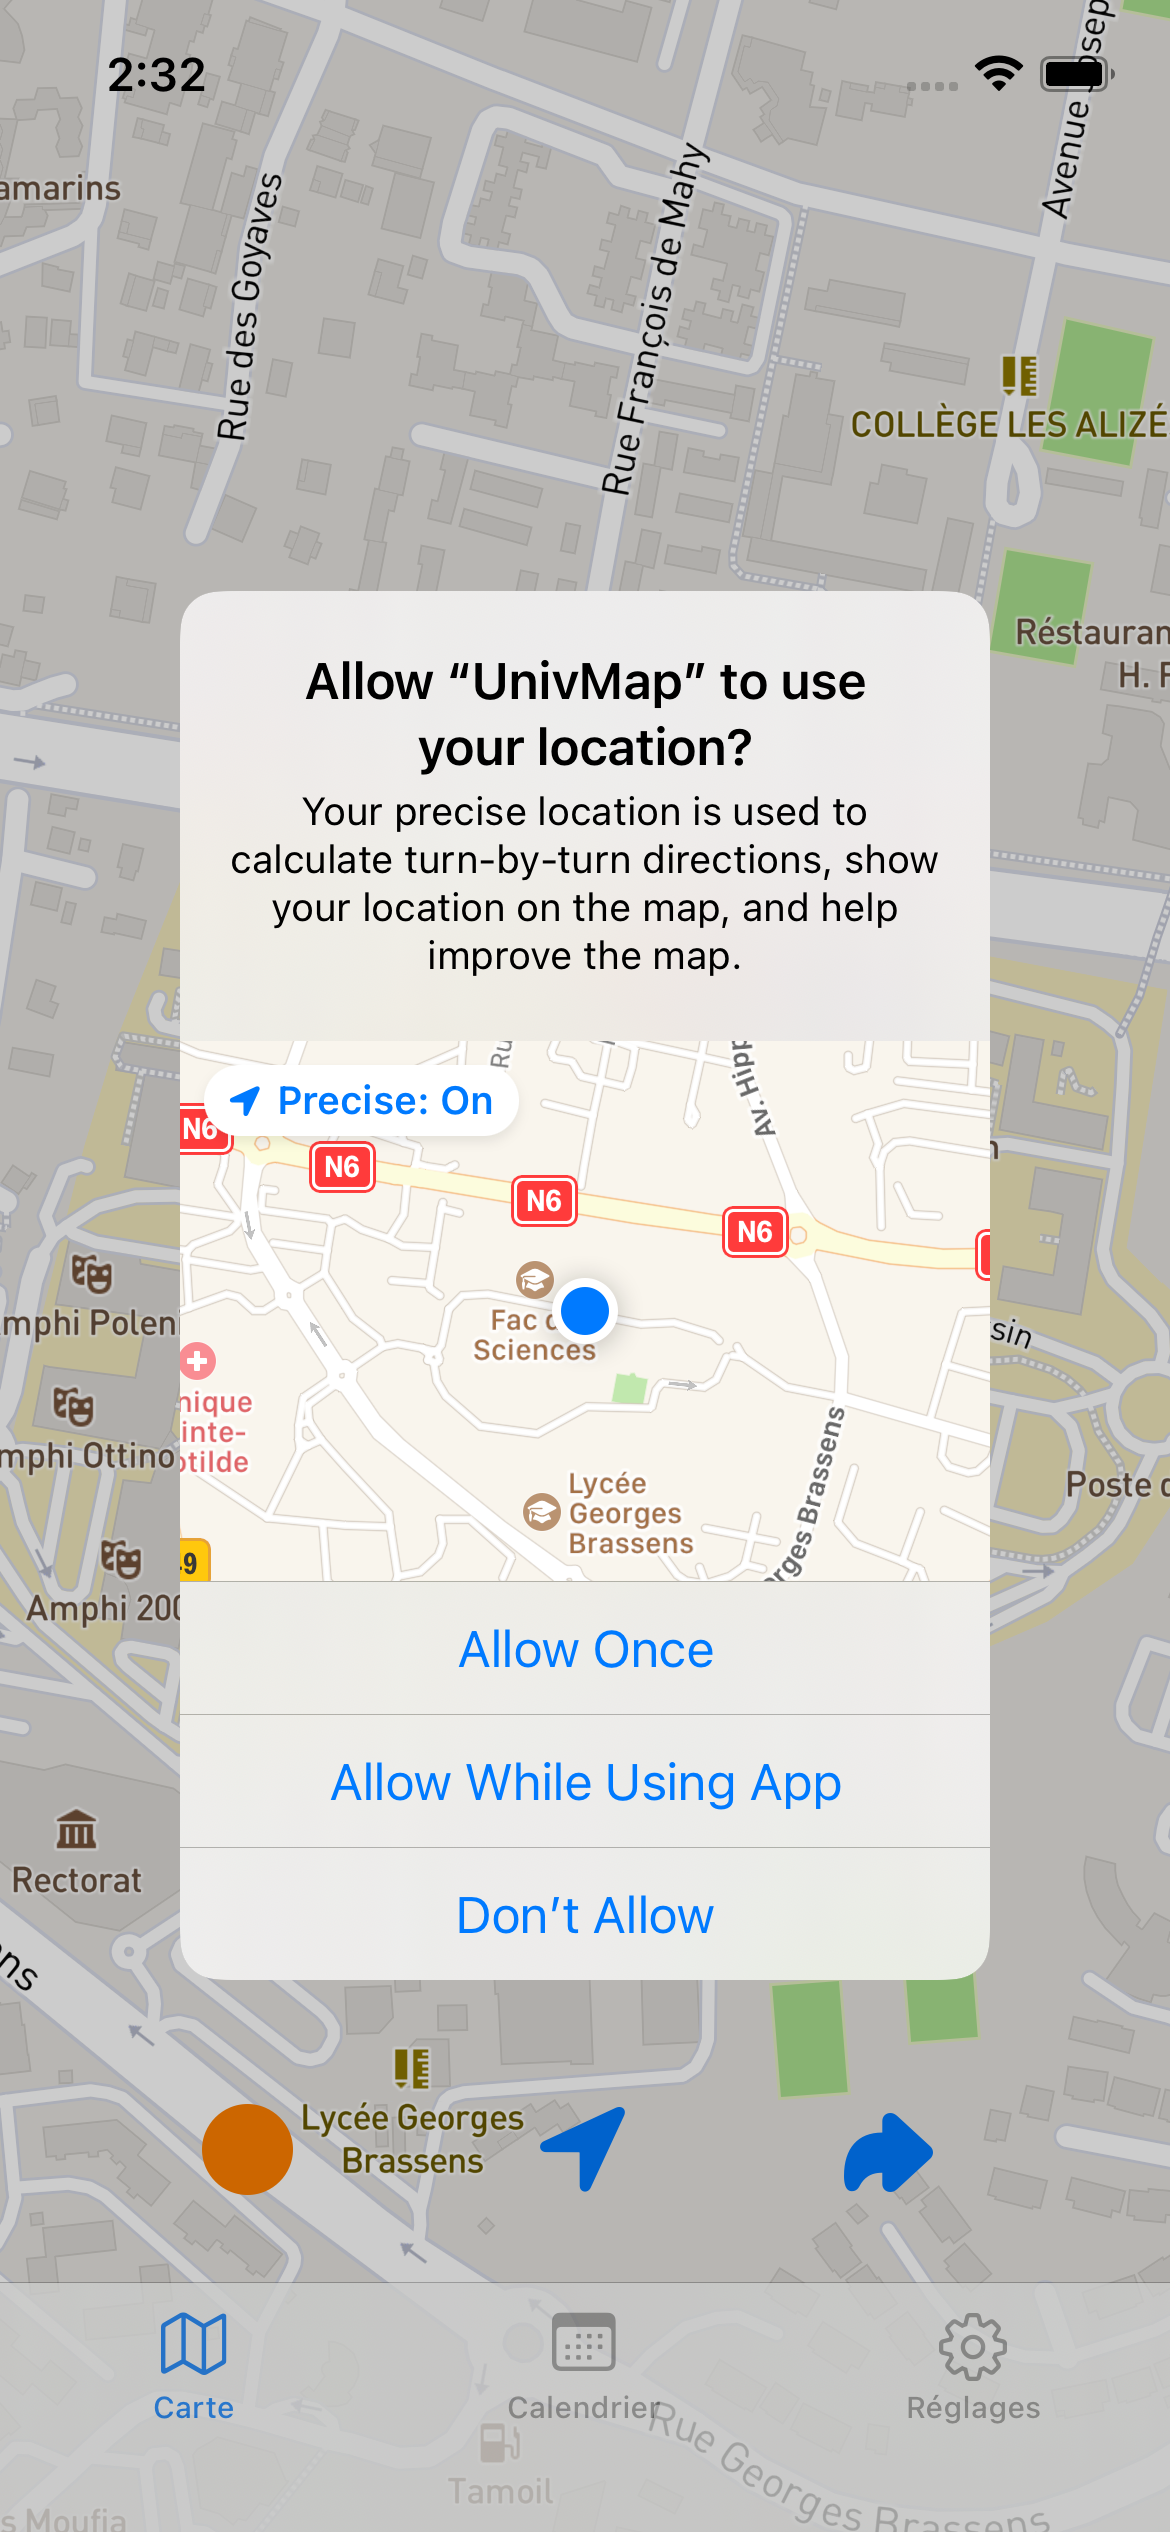
\includegraphics[height=7cm, width=3.5cm, scale=0.5]{allowUserLocation.png}
      \end{tabular} &
      
      \begin{tabular}{l}
          \parbox{0.5\linewidth}{ %  change the parbox width as appropiate
            \textbf{}
              UnivMap requiert une connexion internet afin de localiser la position de l'utilisateur 
          }
      \end{tabular} \\
    \end{tabular}

  \end{frame}

  \begin{frame}
    \frametitle{Comment fontionne : la carte}

    \begin{tabular}{cl}

      \begin{tabular}{c}
        \parbox{0.5\linewidth}{
          \begin{itemize}
            \item Marqueur \textcolor{blue}{BLEU} : cours qui n'ont pas encore débuté
            \item Marqueur \textcolor{orange}{ORANGE} : cours qui débuterons dans moins de 2 heures
            \item Marqueur \textcolor{red}{ROUGE} : cours qui ont déjà commencé
            \item Marqueur \textcolor{gray}{GRIS} : cours terminé
          \end{itemize}
        }
      \end{tabular} &

      \begin{tabular}{l}
        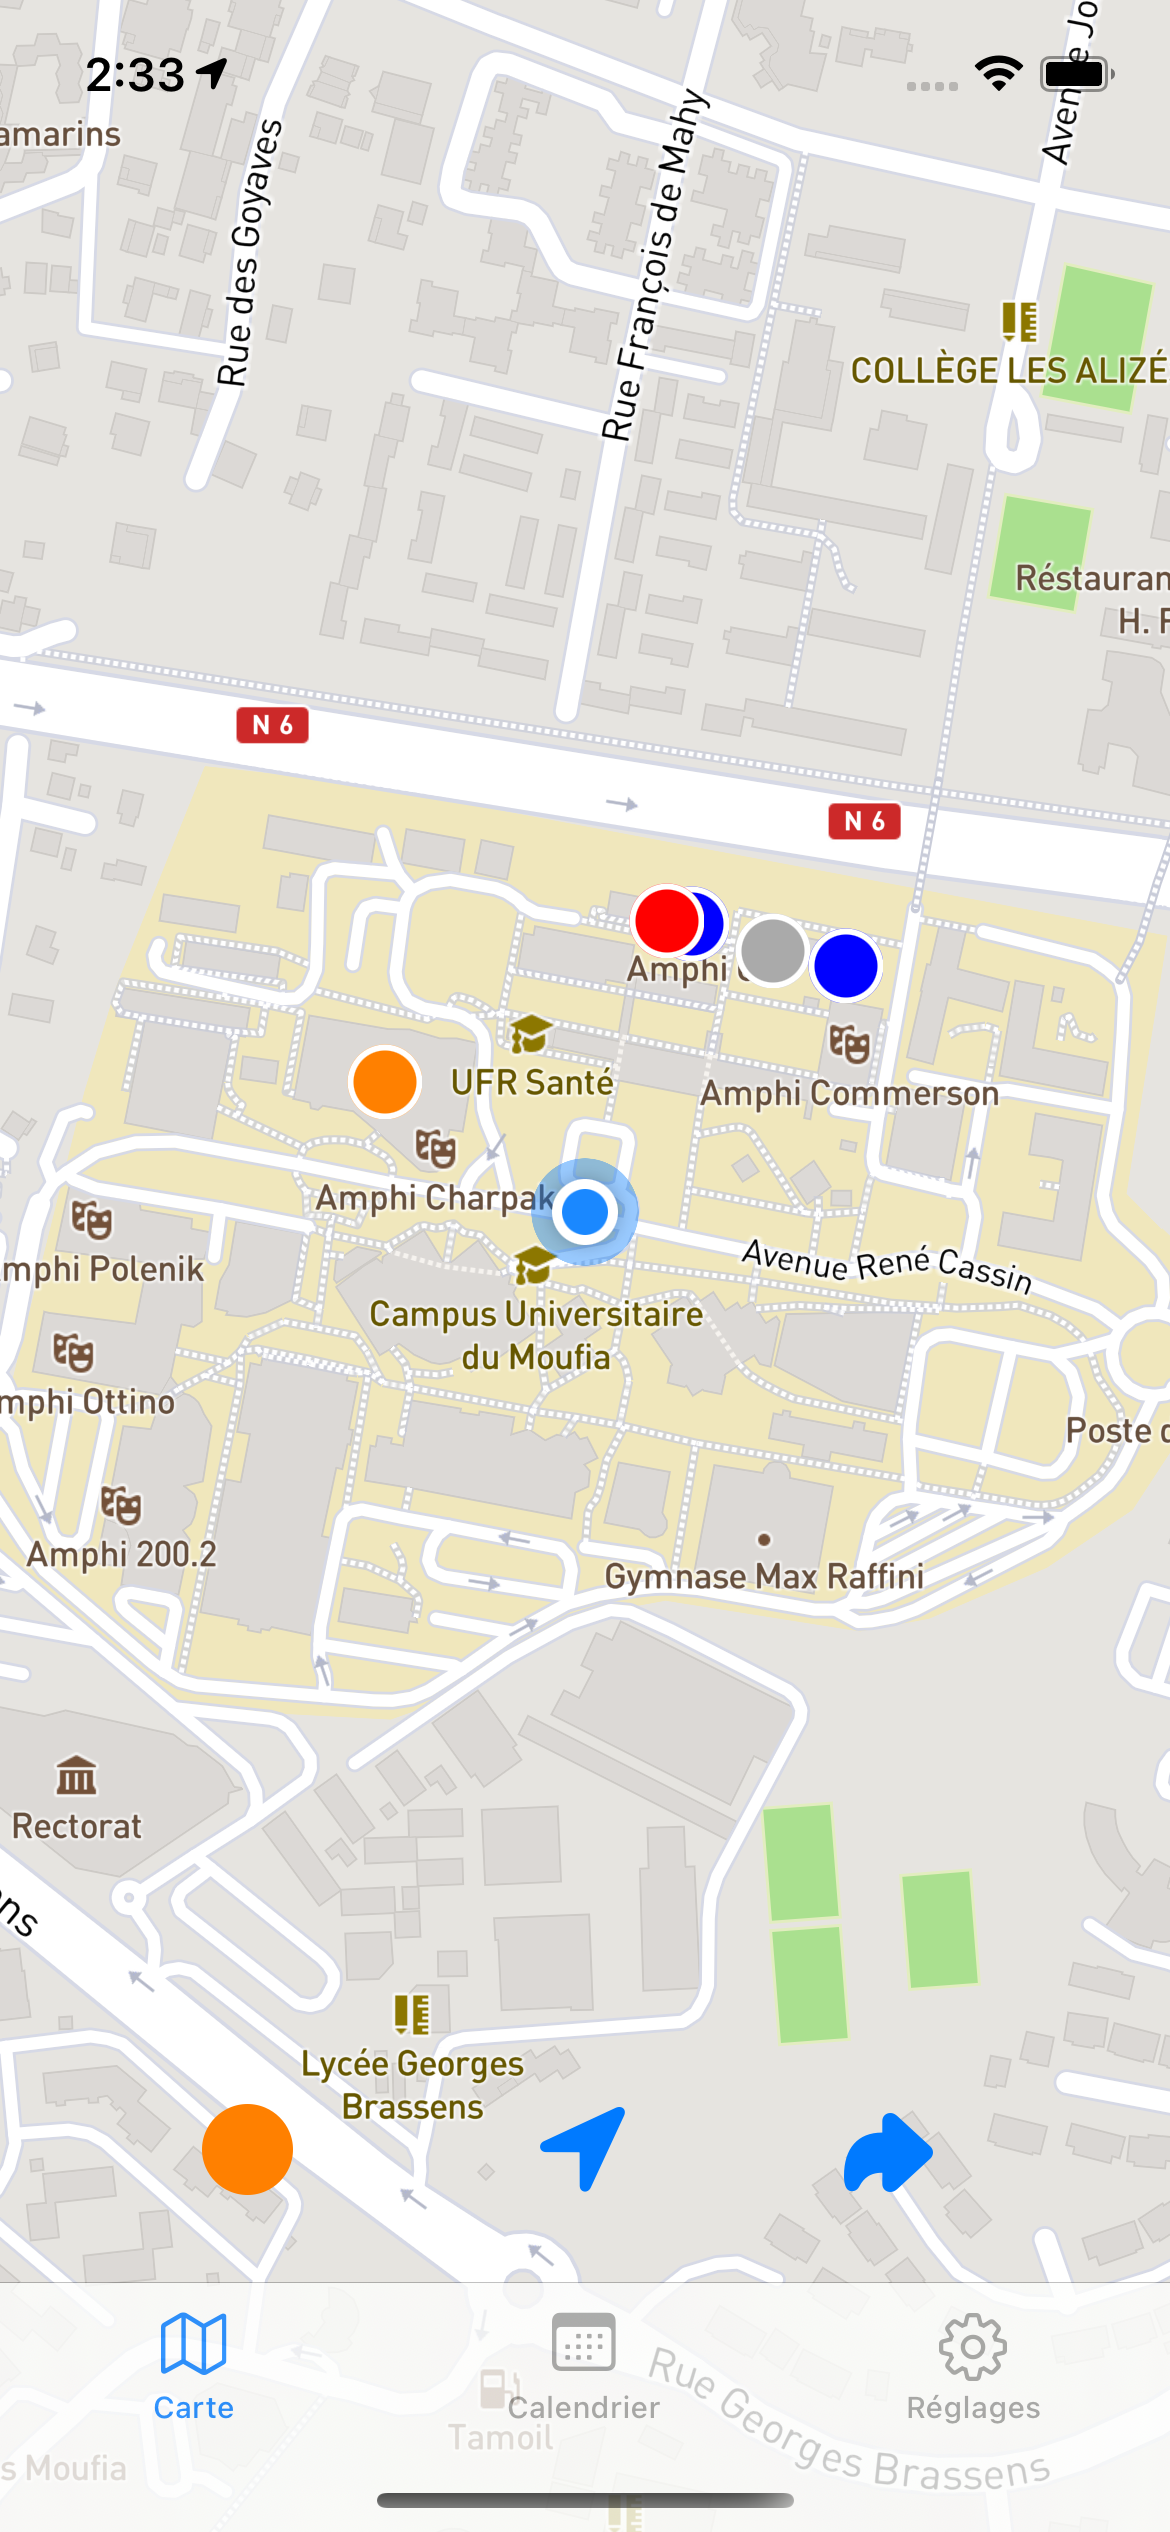
\includegraphics[height=7cm, width=3.5cm, scale=0.5]{map.png}
      \end{tabular}\\

    \end{tabular}

  \end{frame}




  \begin{frame}
    \frametitle{Comment fontionne : la carte}

    \begin{tabular}{cl}

      \begin{tabular}{c}
        \parbox{0.5\linewidth}{
            \textbf{}
            En séléctionnant un marqueur, un pop-up apparait affichant les informations du cours
        }
      \end{tabular} &

      \begin{tabular}{l}
        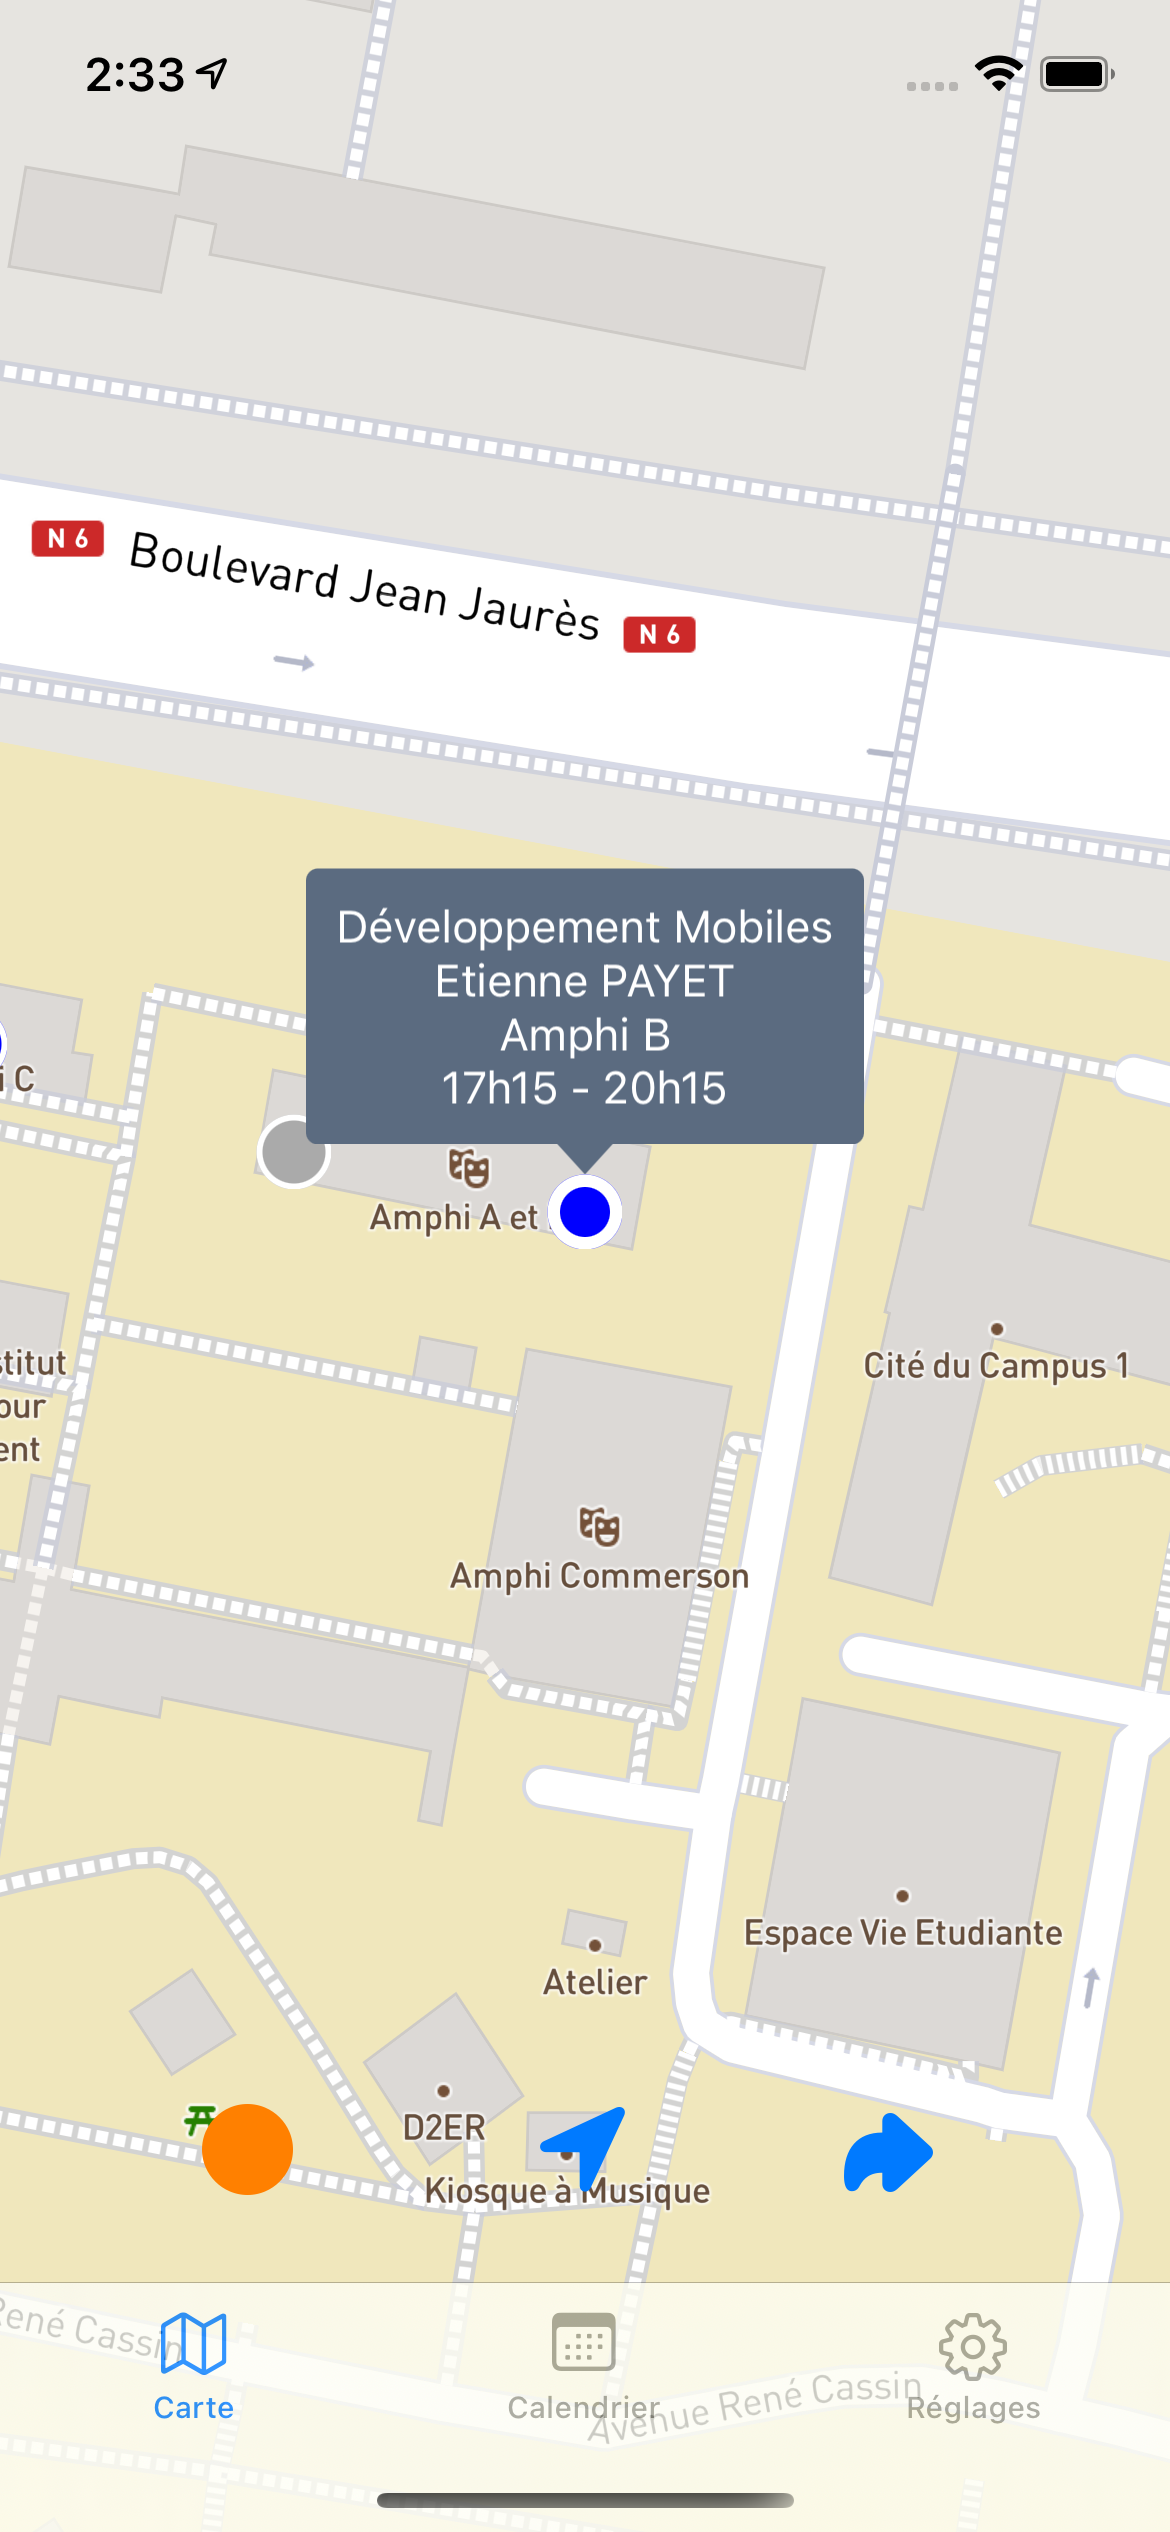
\includegraphics[height=7cm, width=3.5cm, scale=0.5]{point_bleu.png}
      \end{tabular}\\

    \end{tabular}

  \end{frame}




  \begin{frame}
    \frametitle{Architecture du code : le calendrier}

    \begin{tabular}{cl}

      \begin{tabular}{c}
        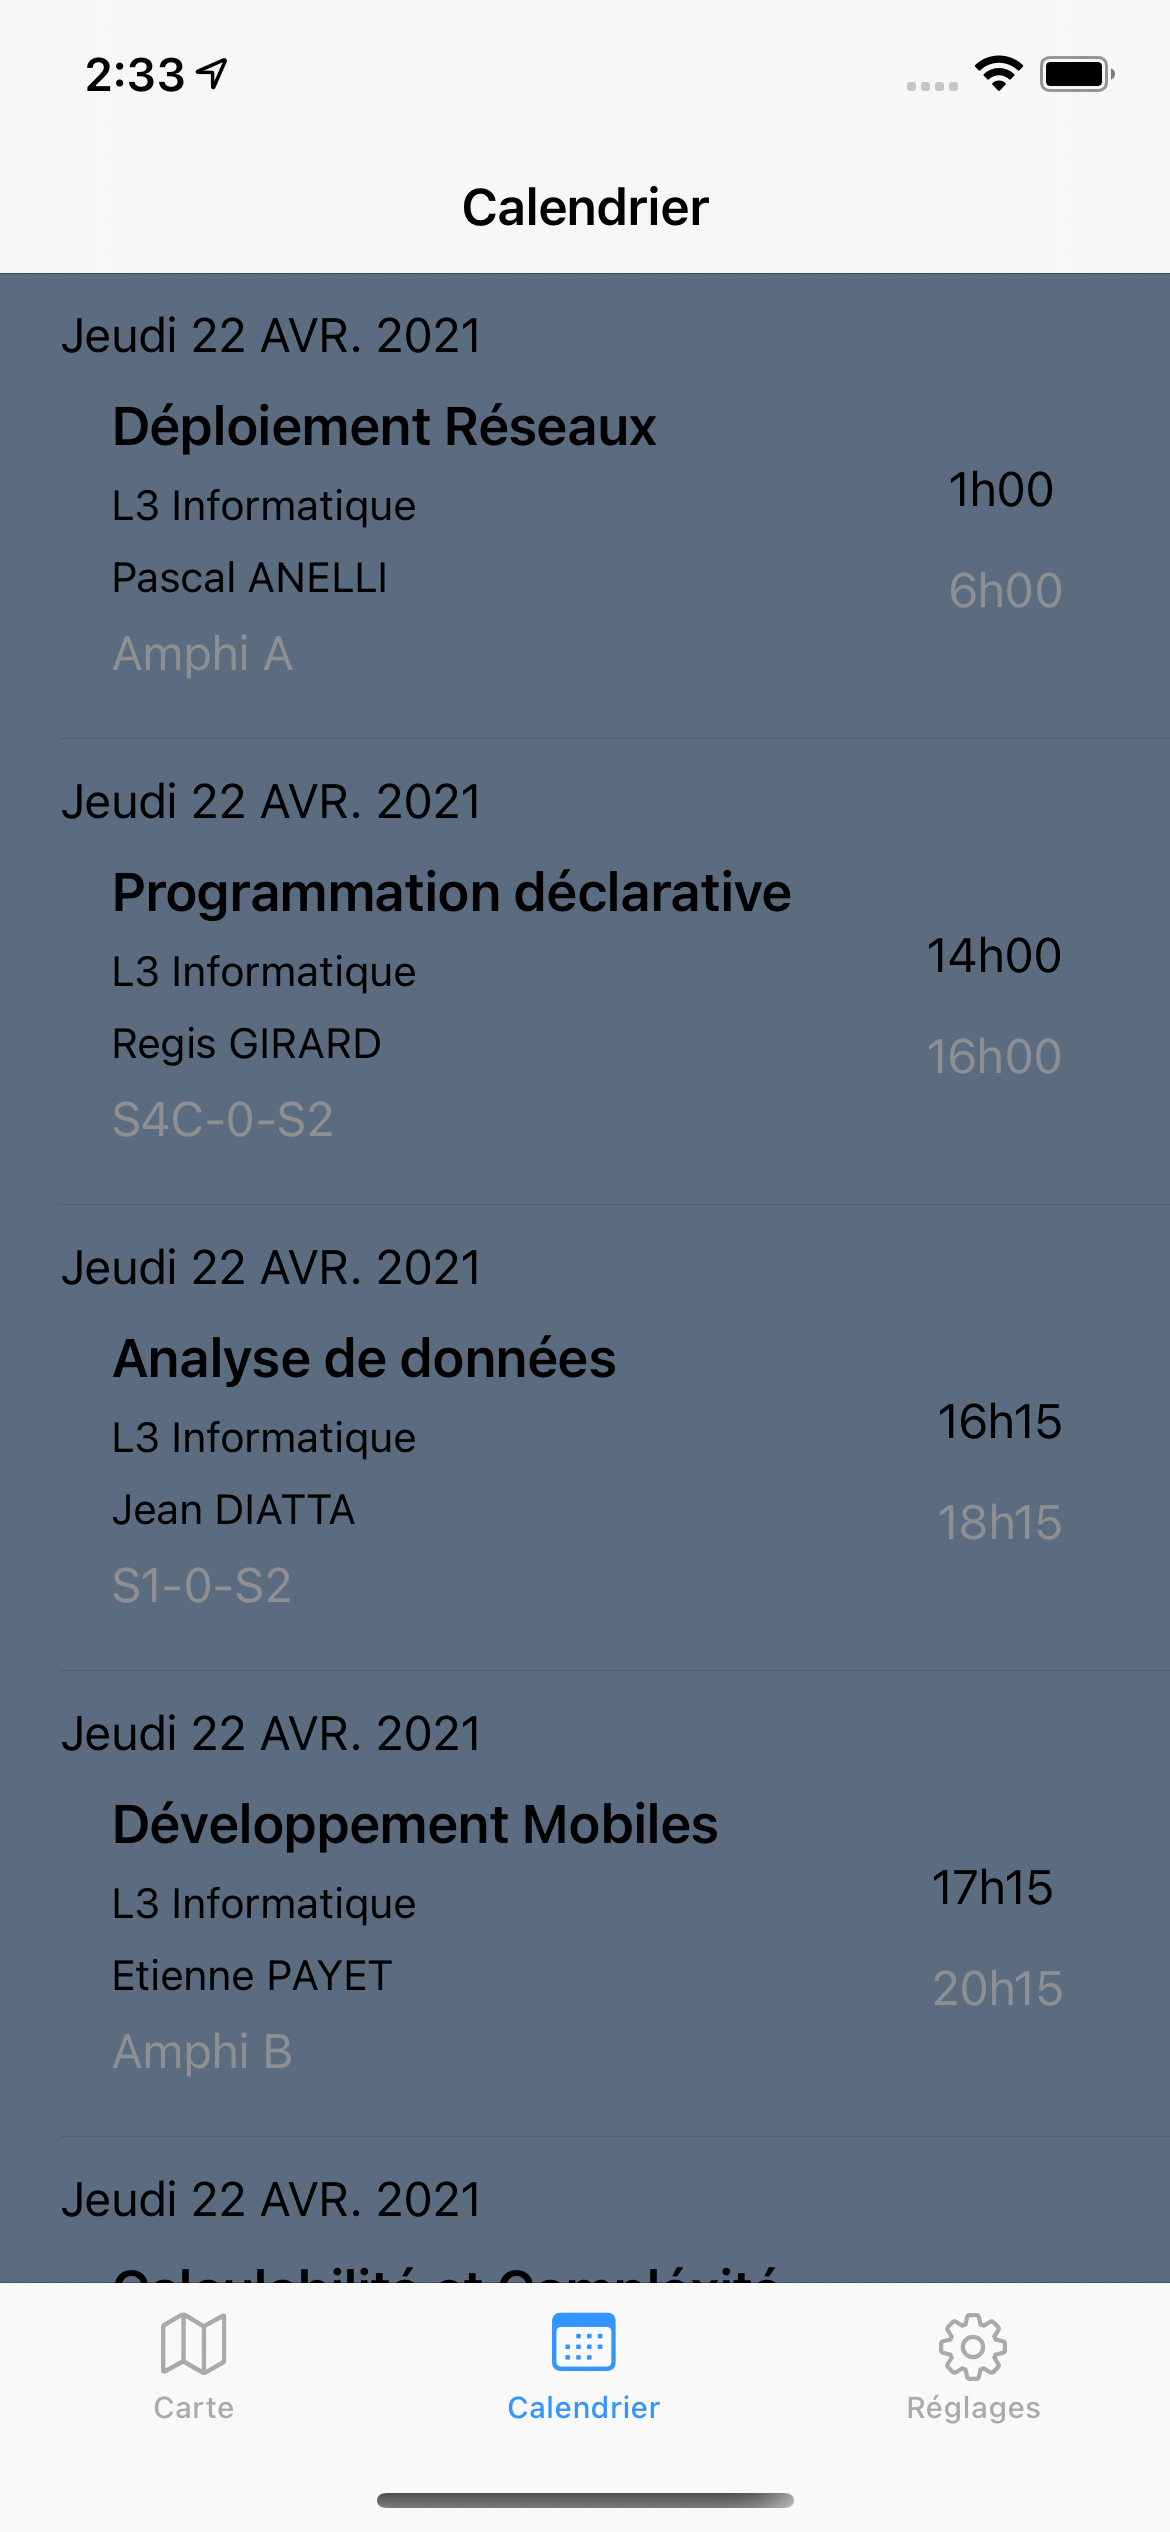
\includegraphics[height=7cm, width=3.5cm, scale=0.5]{calendar.png}
      \end{tabular} &
      
      \begin{tabular}{l}
          \parbox{0.5\linewidth}{
            \textbf{}
              Ici tous les cours sont affichés, trier par ordre croissant selon l'heure
          }
      \end{tabular} \\
    \end{tabular}

  \end{frame}

  \begin{frame}
    \frametitle{Architecture du code : le calendrier}

    \begin{tabular}{cl}

      \begin{tabular}{c}
        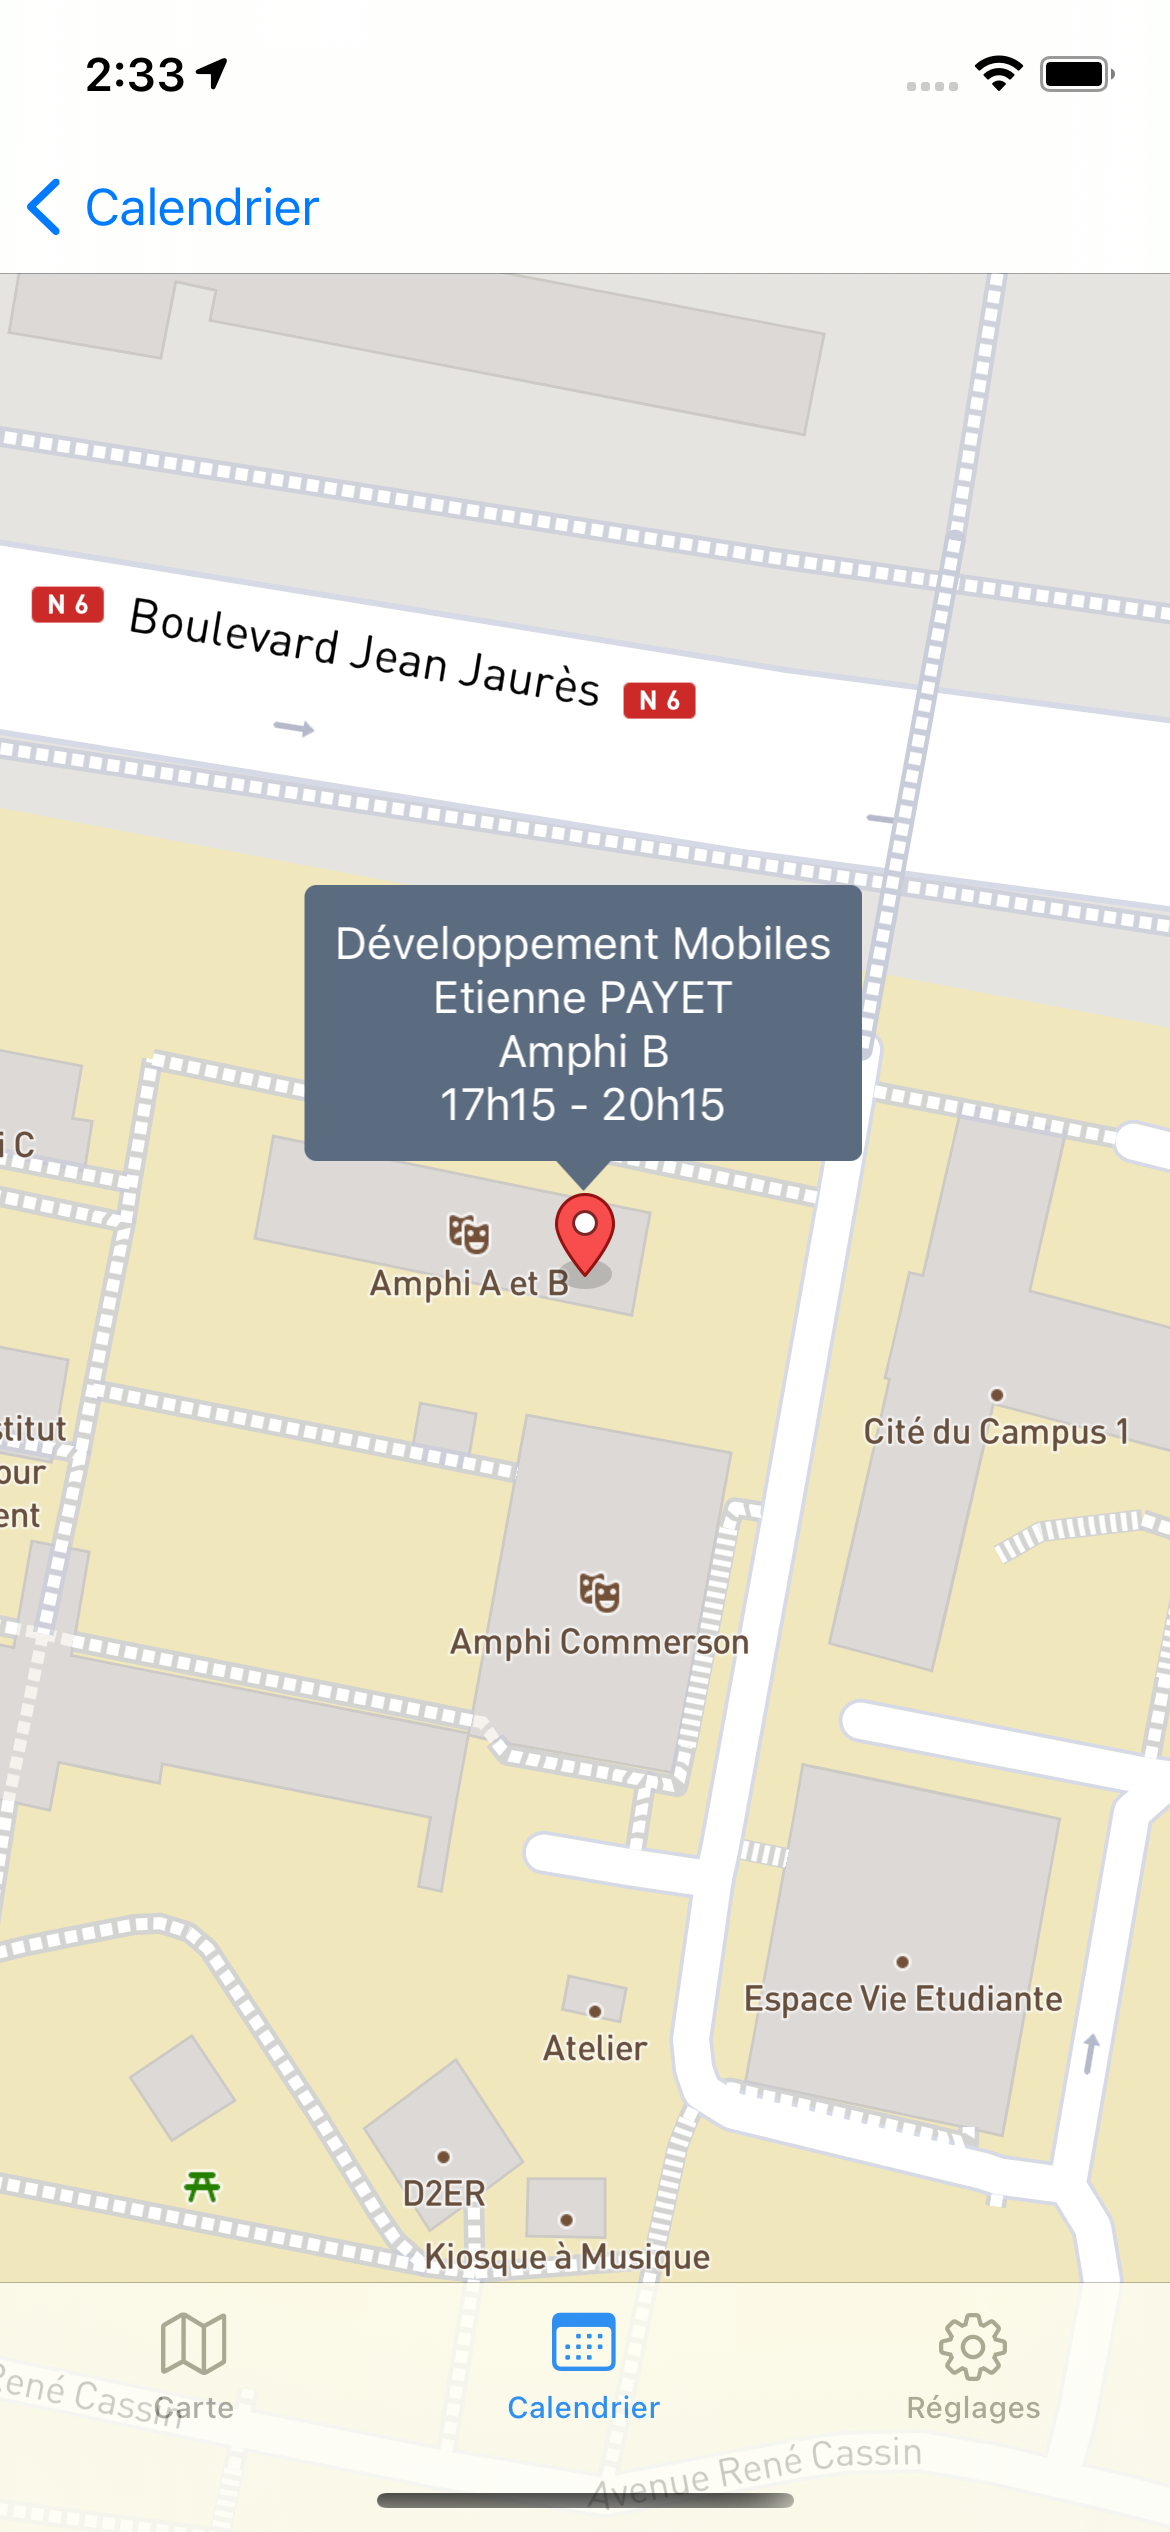
\includegraphics[height=7cm, width=3.5cm, scale=0.5]{calendar_position.png}
      \end{tabular} &
      
      \begin{tabular}{l}
          \parbox{0.5\linewidth}{
            \textbf{}
              En cliquant sur un cours, l'utilisateur est redirigé vers une autre vue affichant la position du cours.
          }
      \end{tabular} \\
    \end{tabular}

  \end{frame}





  \begin{frame}
    \frametitle{Introduction}
    \begin{center}
      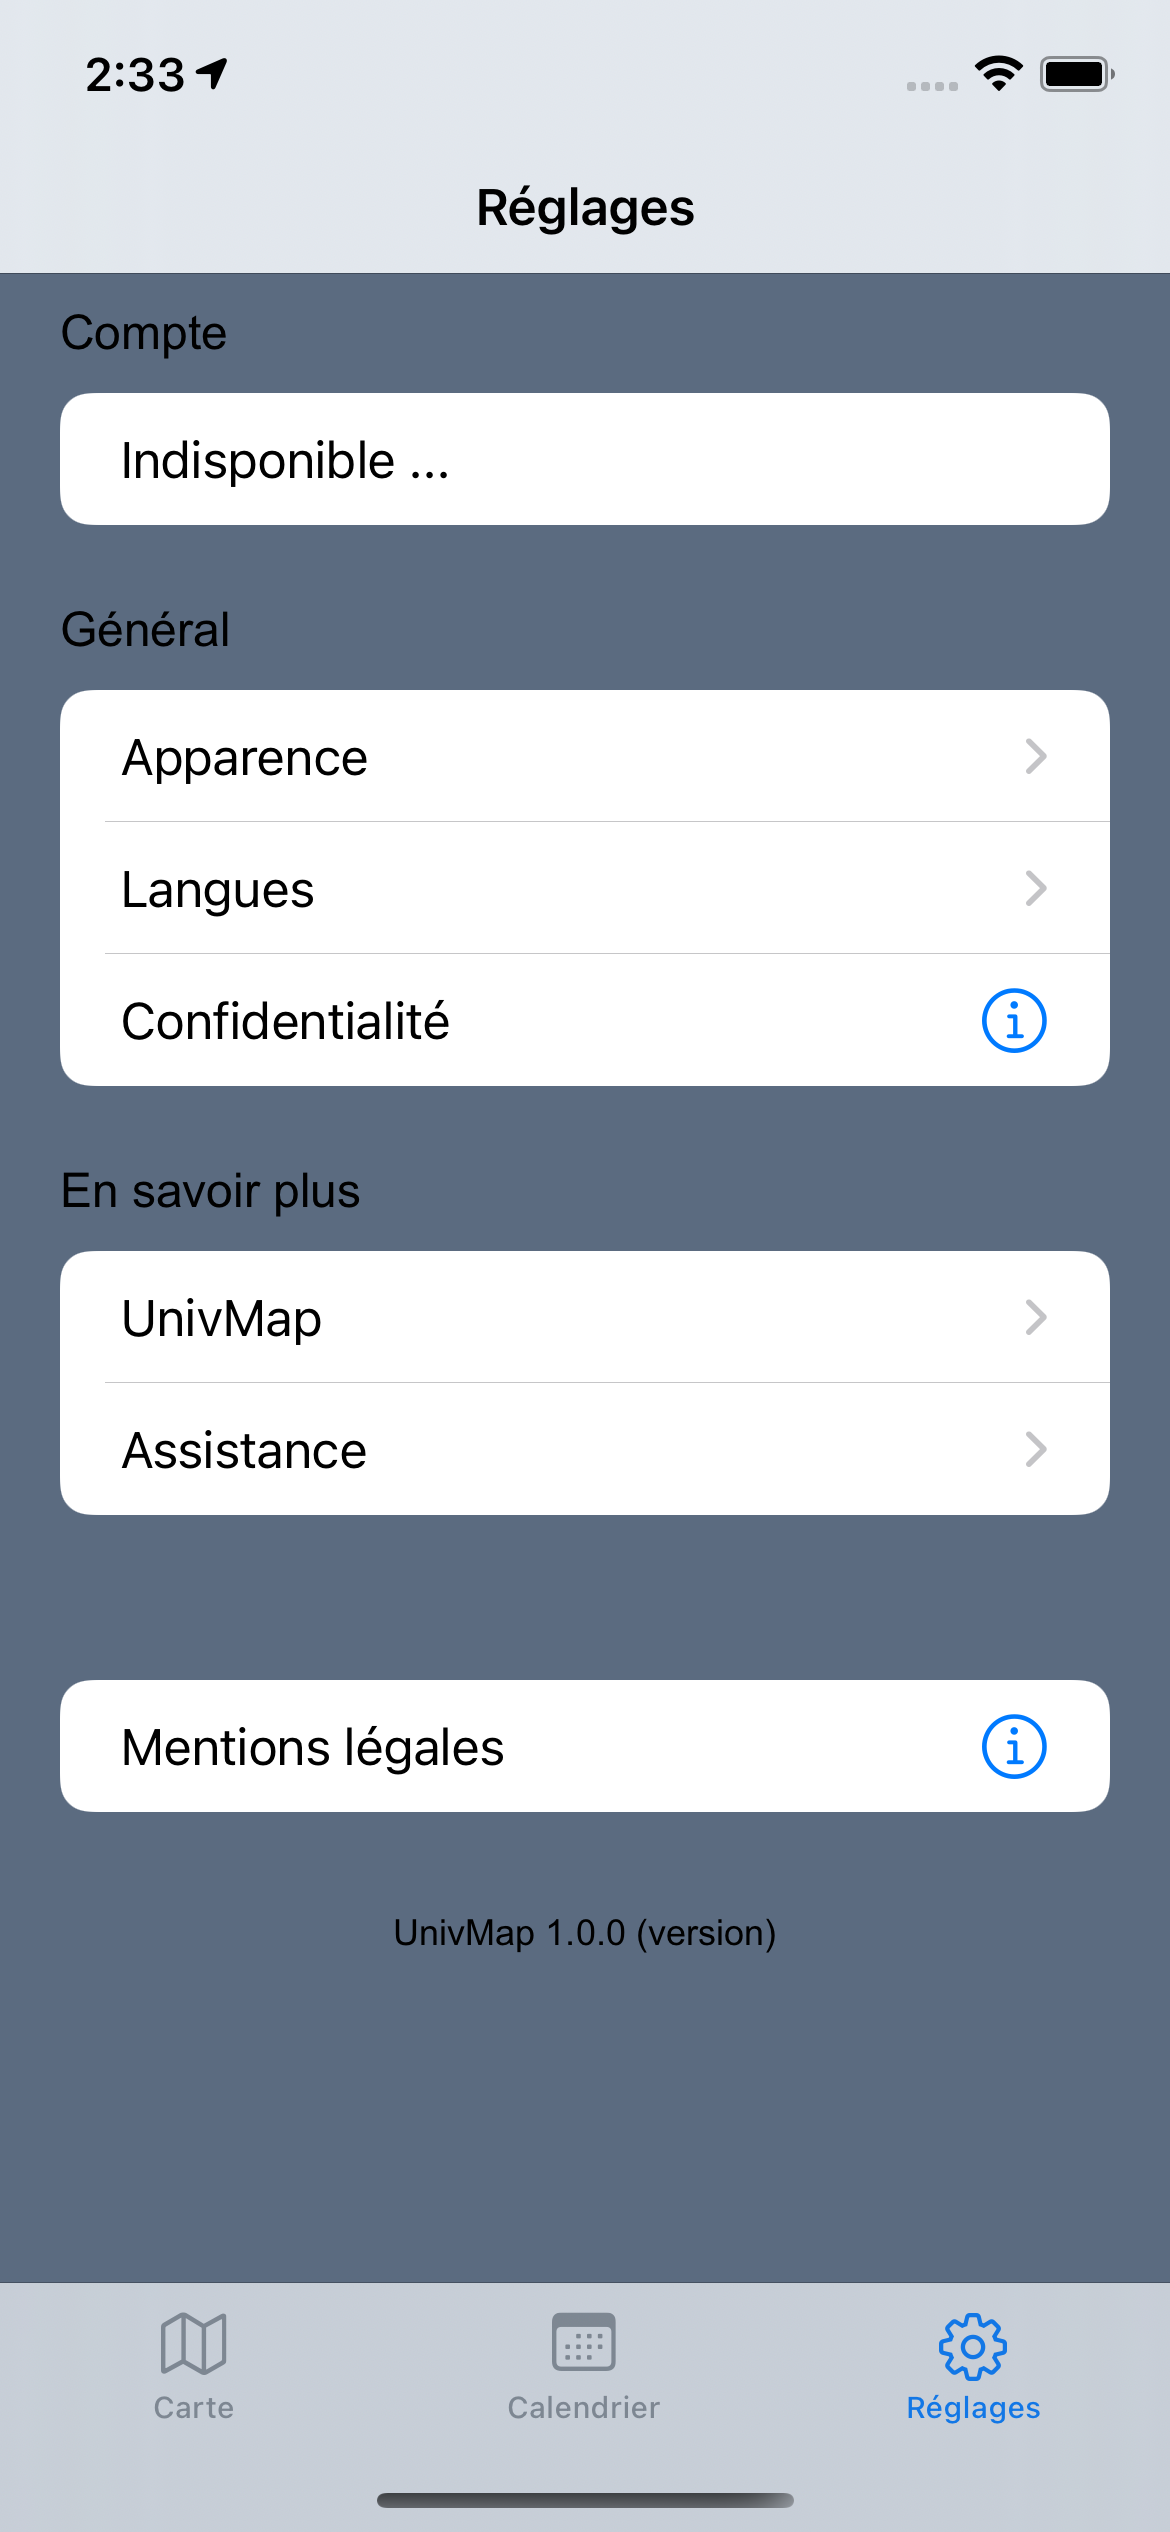
\includegraphics[width=35mm, scale=0.5]{setting.png}
      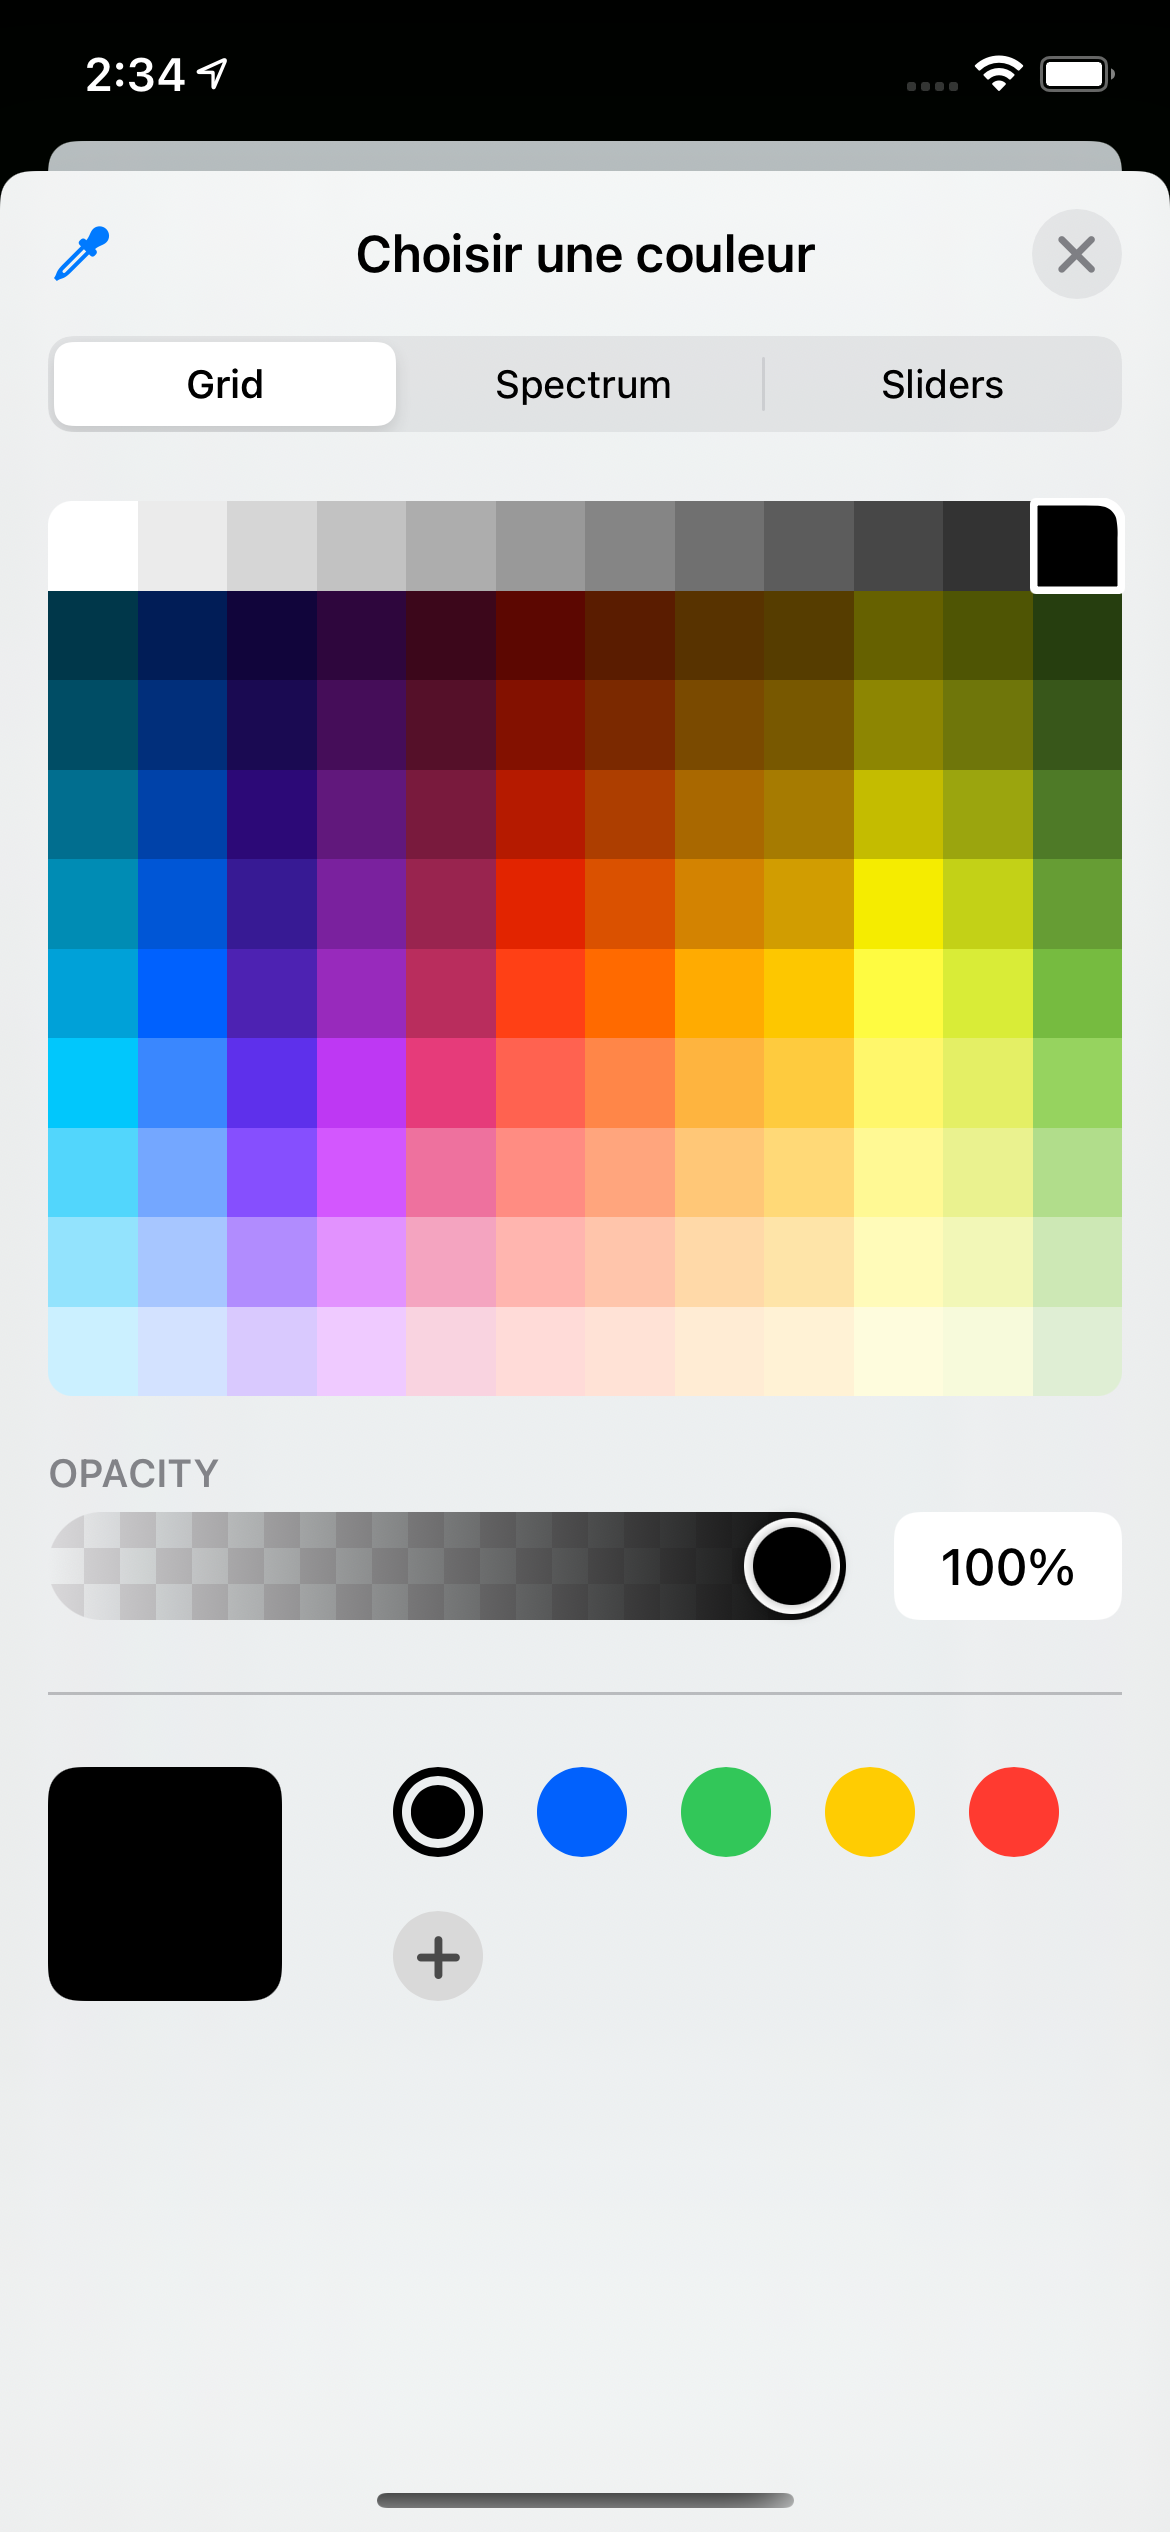
\includegraphics[width=35mm, scale=0.5]{setting_appearance.png}
      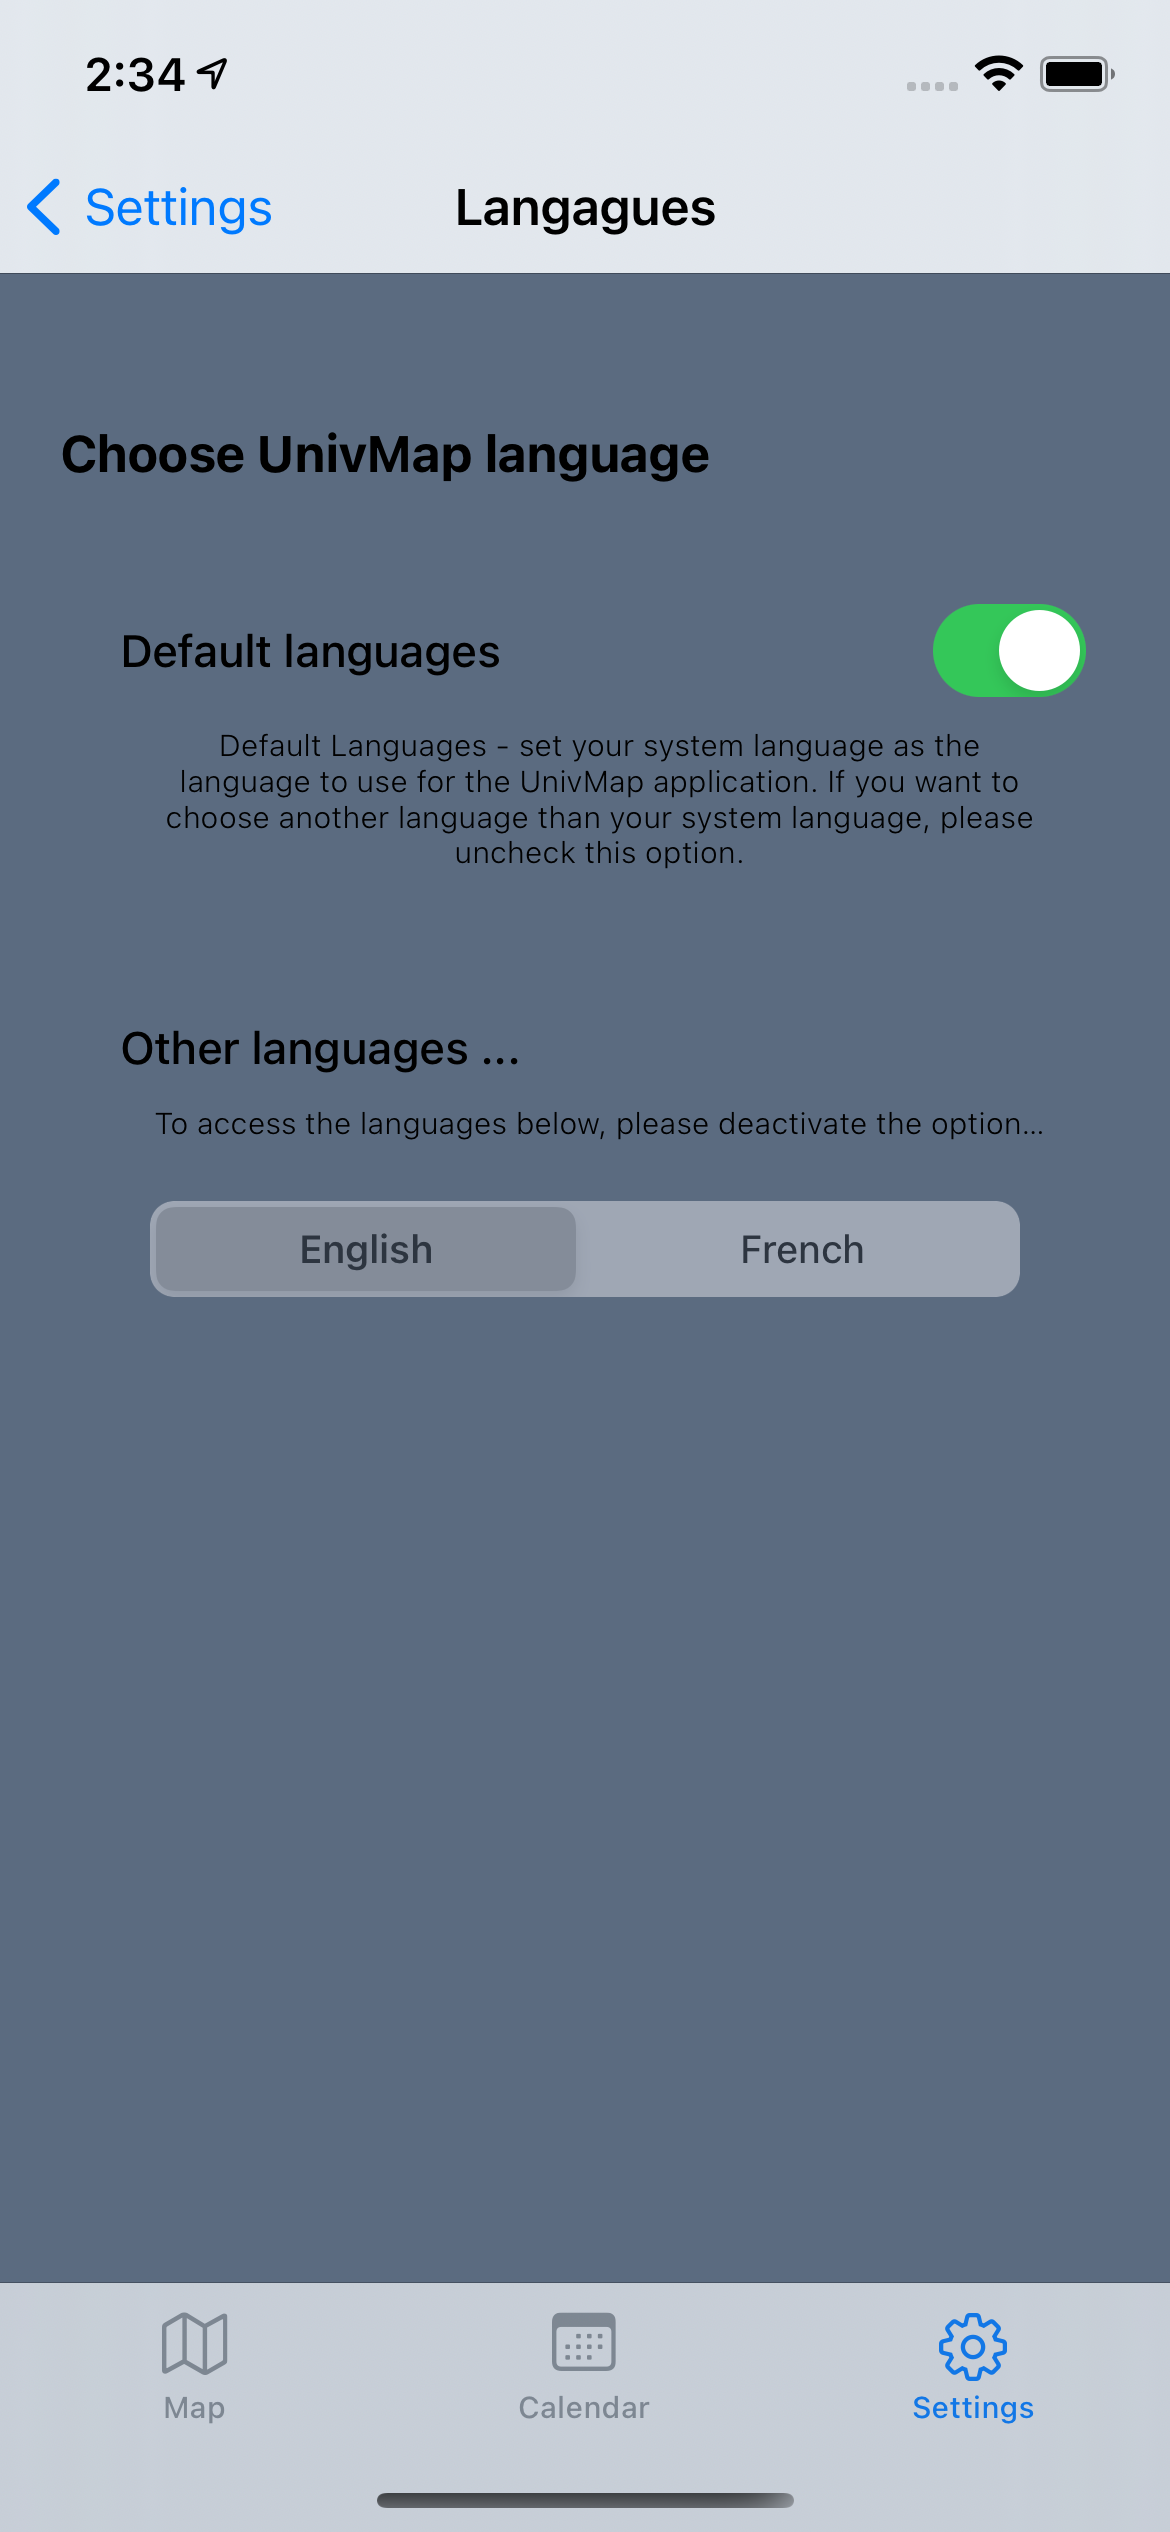
\includegraphics[width=35mm, scale=0.5]{setting_languageOn.png}
    \end{center}
    
  \end{frame}






% ****************************************************************************************************************************************
% *************************************                      Architecture du code                      ***********************************
% ****************************************************************************************************************************************
%
%
%%%%%%%%%%%%%%%%%%%%%%%%%%%%%%%%%%%%%%%%%%%%%%%%%%%%%%%%%%%%%%%%%%%%%%%%%%%%%
\section{Architecture du code}
%%%%%%%%%%%%%%%%%%%%%%%%%%%%%%%%%%%%%%%%%%%%%%%%%%%%%%%%%%%%%%%%%%%%%%%%%%%%%
%
%

% ========================= Firebase ==========================================
\subsection{Firebase}
  \begin{frame}
    \frametitle{Firebase : c'est quoi ?}

    \begin{itemize}
      \item Services d'hébergement pour tout type d'application
      \item Racheté par Google en 2014
      \item Firebase : NoSQL
      \item Utilisé par plus de 110 000 développeurs :
      \begin{itemize}
        \item Shazam (iOS et Android)
        \item Le Figaro (iOS et Android)
        \item ...
      \end{itemize}
    \end{itemize}

  \end{frame}

  \begin{frame}
    \frametitle{Firebase : c'est quoi ?}

    \begin{center}
      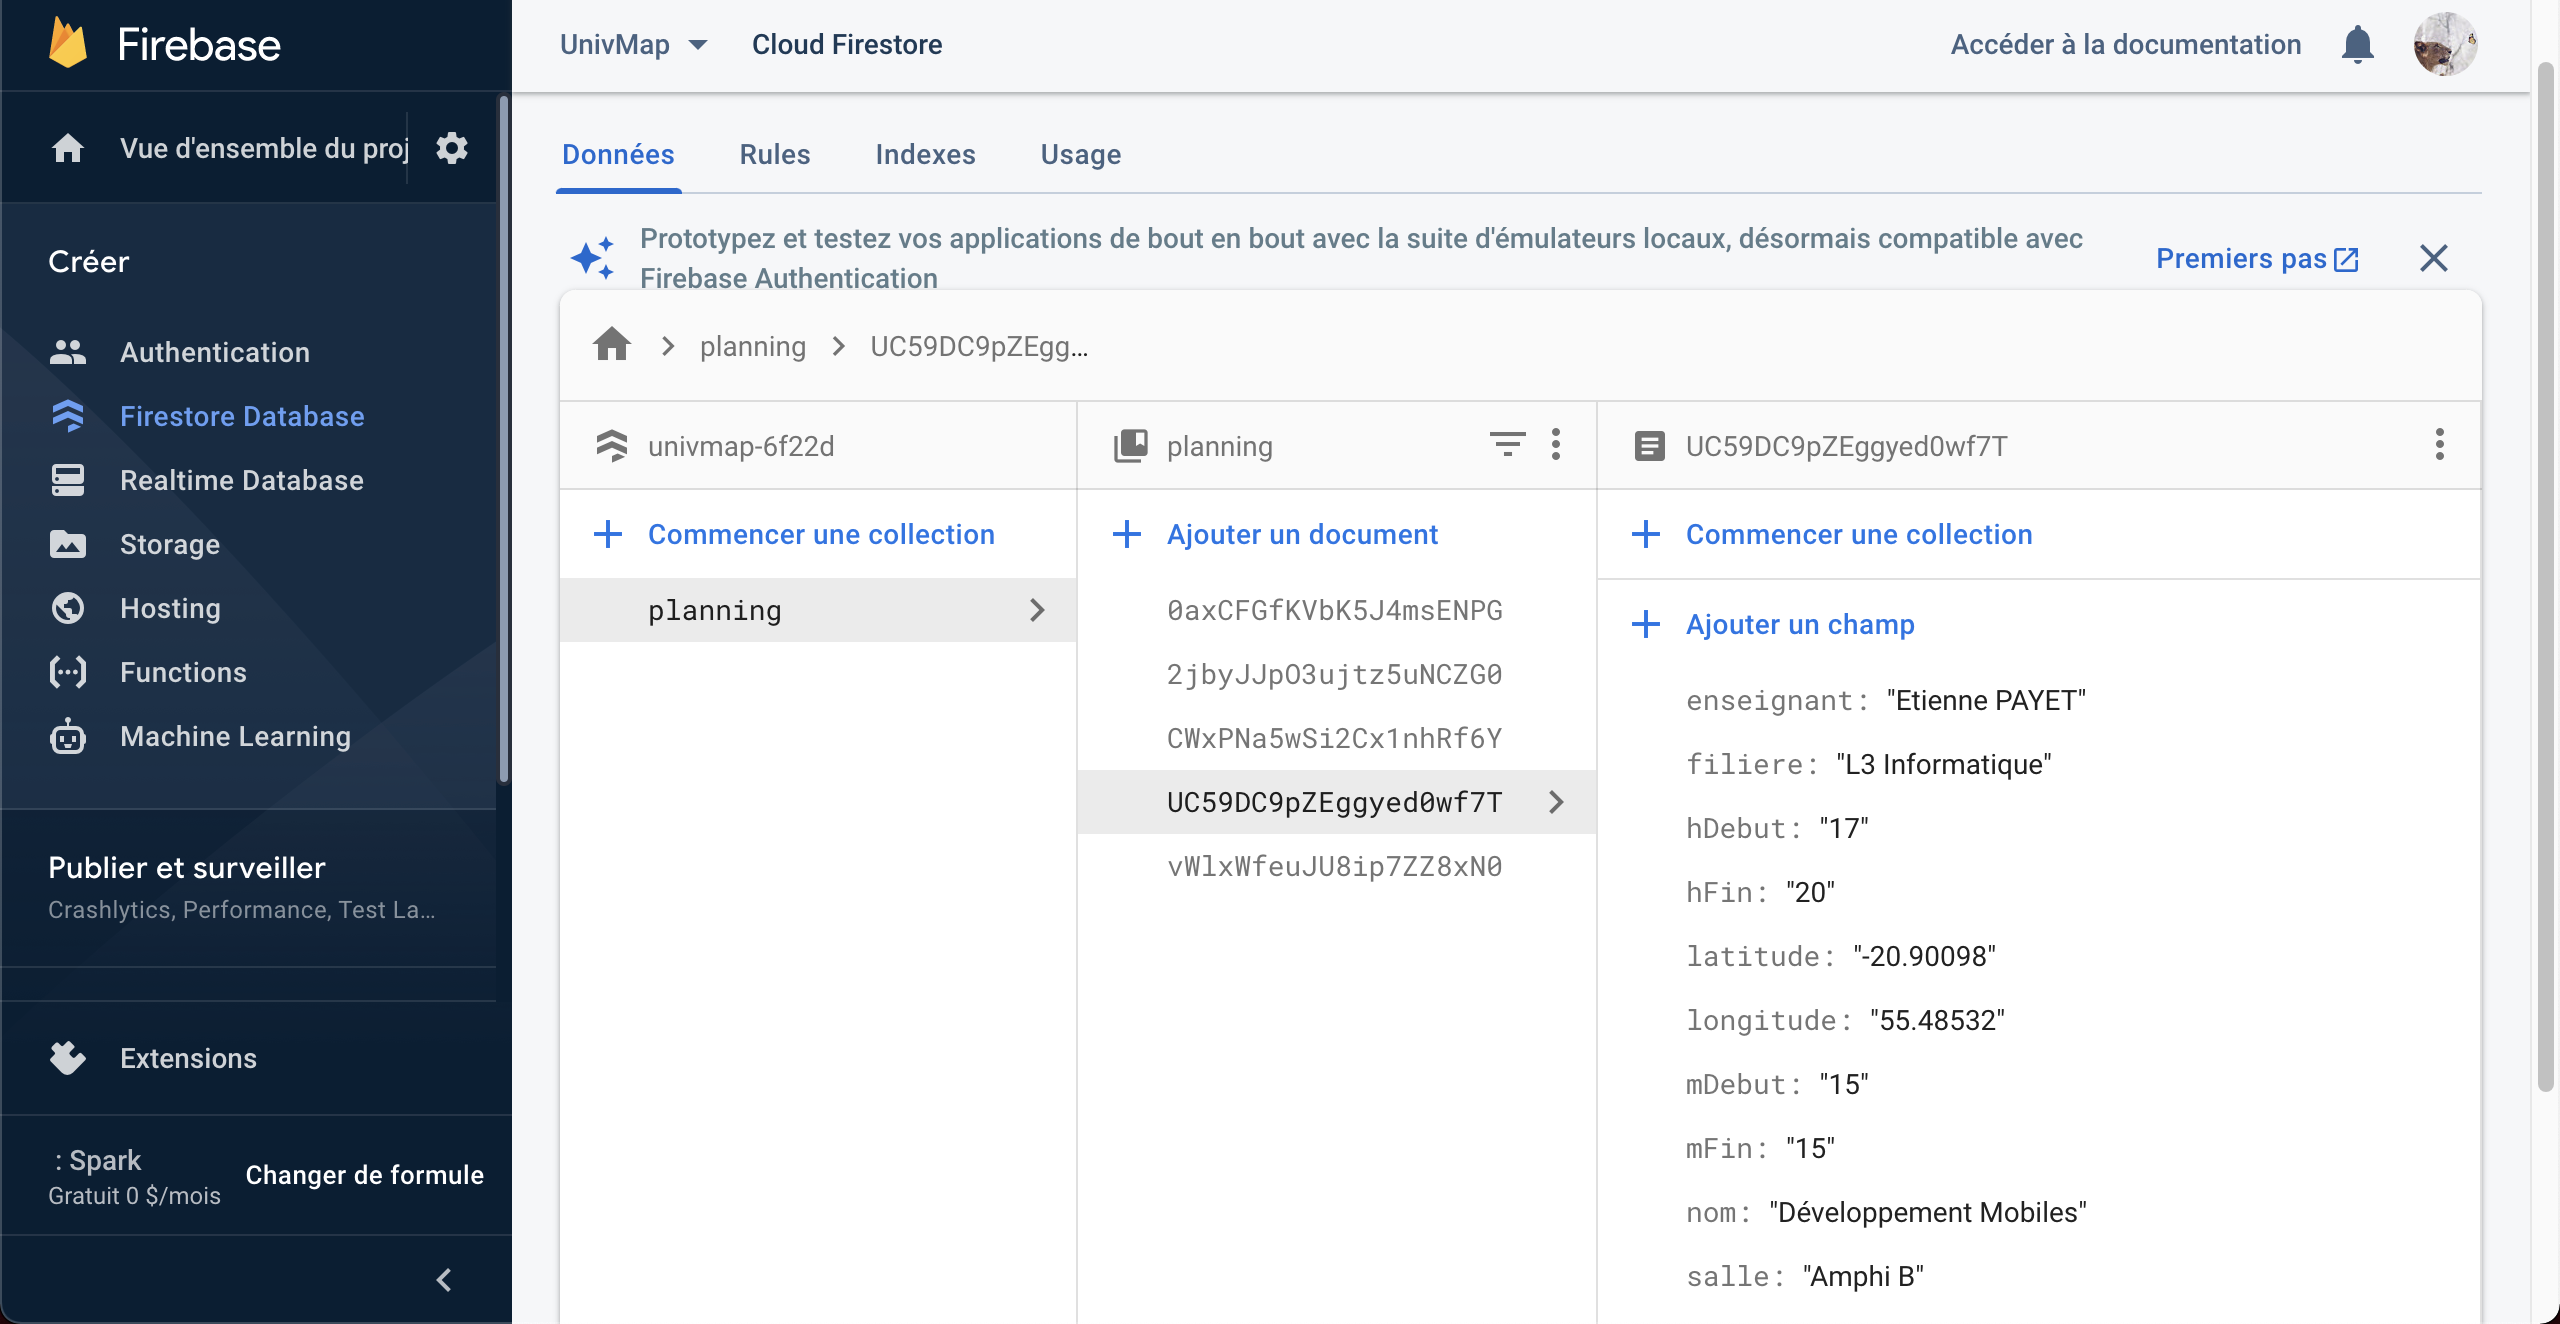
\includegraphics[width=120mm, scale=0.5]{firebase.png}
    \end{center}

  \end{frame}

  \begin{frame}
    \frametitle{Architecture du code : Firebase}

    \begin{center}
      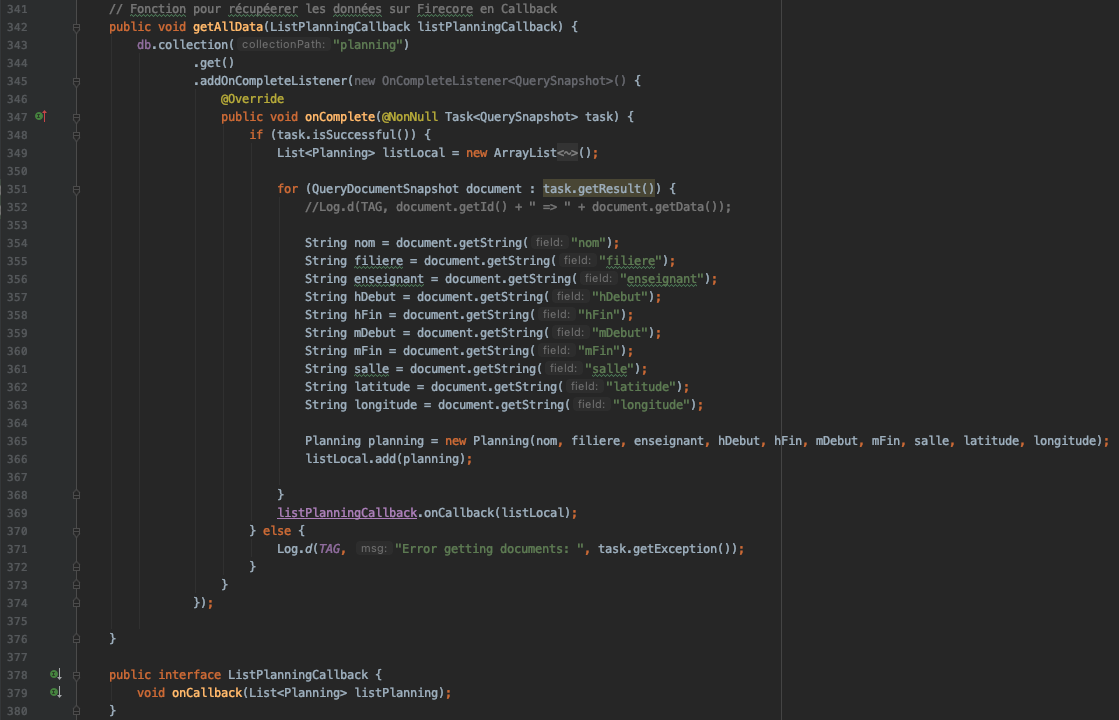
\includegraphics[width=120mm, scale=0.5]{getAllData-firebase.png}
    \end{center}

  \end{frame}




% ========================= Mapbox ==========================================
\subsection{Mapbox}
  \begin{frame}
    \frametitle{Mapbox : c'est quoi ?}

    \begin{itemize}
      \item Entreprise américaine spécialisée dans la cartographie en ligne
      \item Mapbox reposent principalement sur le logiciel libre et sur les données d'OpenStreetMap
      \item Fournis ses services notamment à :
      \begin{itemize}
        \item Pinterest
        \item Le Monde
        \item Snapchat
        \item ...
      \end{itemize}
    \end{itemize}

  \end{frame}

  \begin{frame}
    \frametitle{Architecture du code : Mapbox}

    \begin{center}
      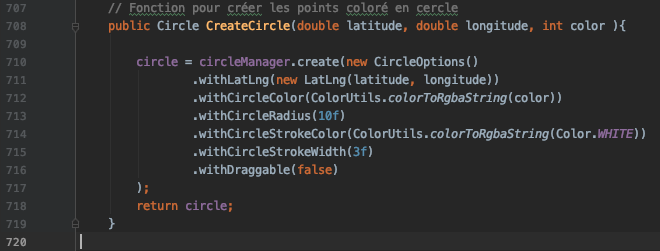
\includegraphics[width=120mm, scale=0.5]{circle.png}
    \end{center}

  \end{frame}

  \begin{frame}
    \frametitle{Architecture du code : Mapbox}

    \begin{center}
      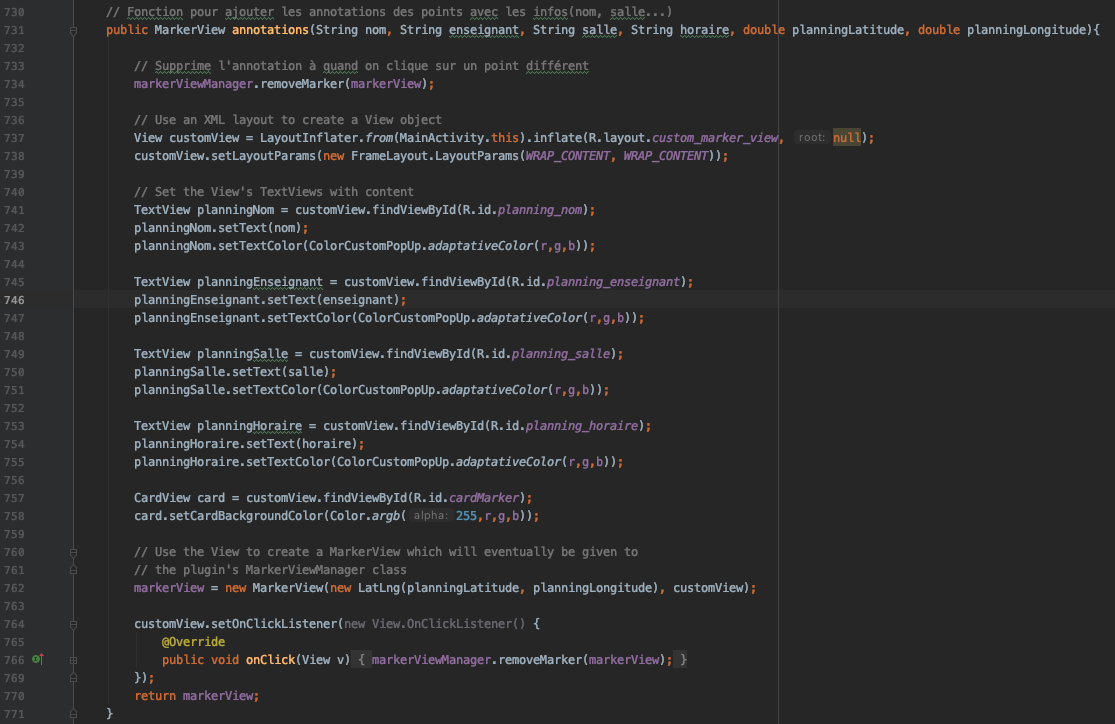
\includegraphics[width=120mm, scale=0.5]{markerView.png}
    \end{center}

  \end{frame}

  


% ========================= Paramètres ==========================================
  \begin{frame}
    \frametitle{Architecture du code : les paramètres}

    \begin{tabular}{cl}

      \begin{tabular}{c}
        \parbox{0.5\linewidth}{
          \begin{itemize}
            \item Une liste d'options en TableViewController(iOS) et listView(Android)
            \item Sélection d'une option redirige vers une nouvelle View/Activity
          \end{itemize}
        }
      \end{tabular} &
      
      \begin{tabular}{l}
        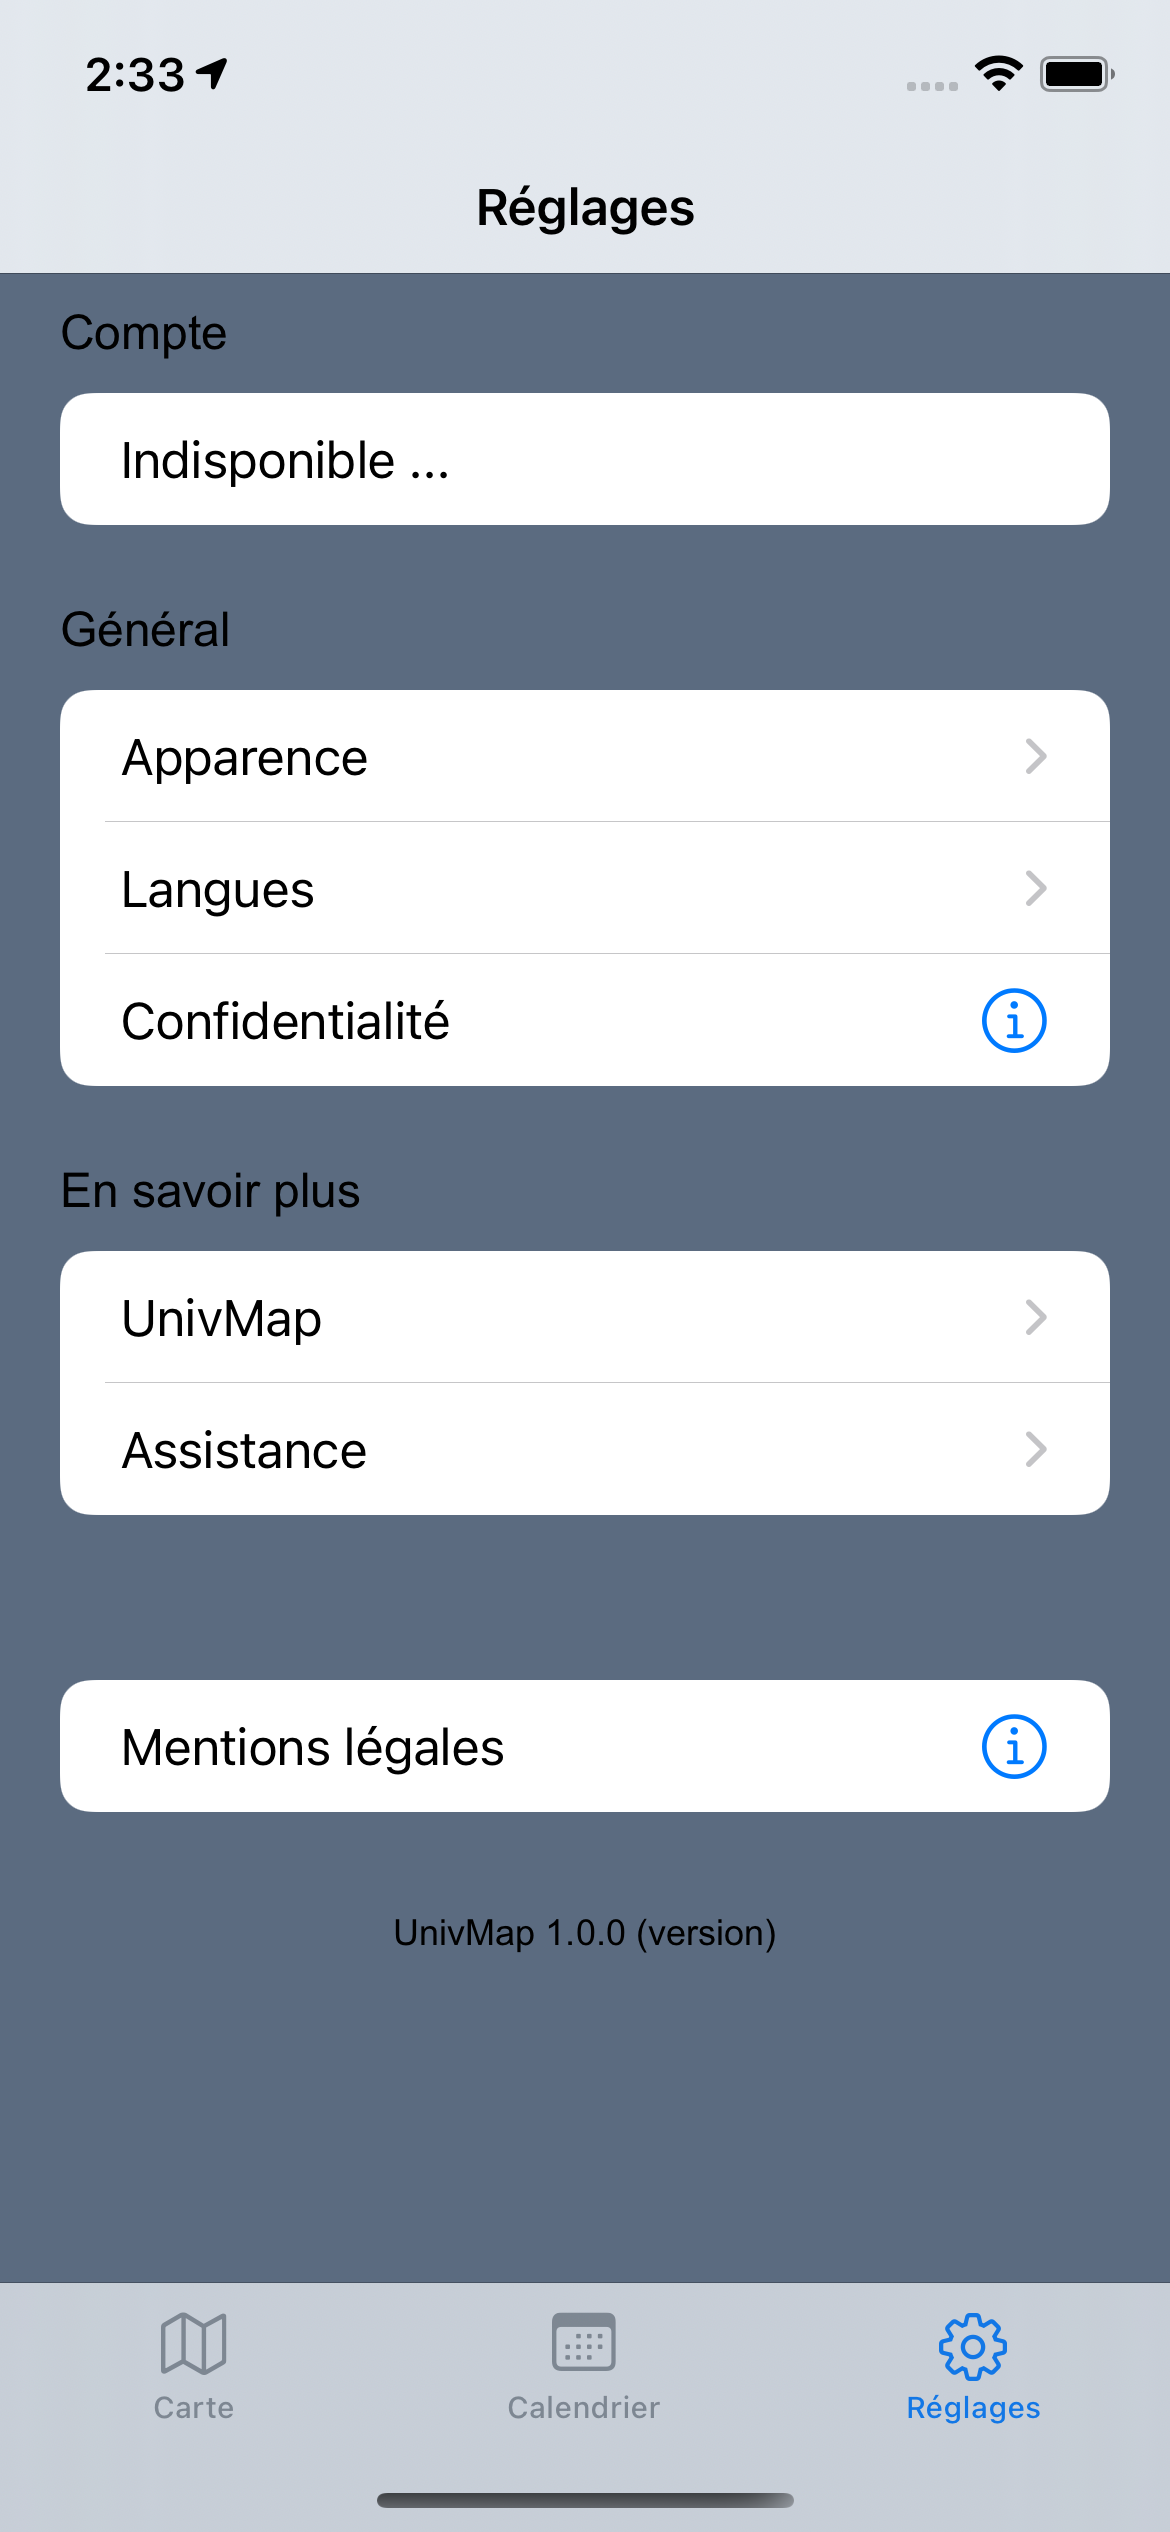
\includegraphics[height=7cm, width=3.5cm, scale=0.5]{setting.png}
      \end{tabular} \\
    \end{tabular}
  \end{frame}



\subsection{Paramètres : apparence}
  \begin{frame}
    \frametitle{Architecture du code : apparence}

    \begin{tabular}{cl}

      \begin{tabular}{c}
        \parbox{0.5\linewidth}{
          \begin{itemize}
            \item Utilisation du colorPickerViewController
            \item Changement de couleur de chaque Views grâce à la persistance de donnée\\
            (UserDefaults(iOS)/\\SharedPreferences(Android))
          \end{itemize}
        }
      \end{tabular} &
      
      \begin{tabular}{l}
        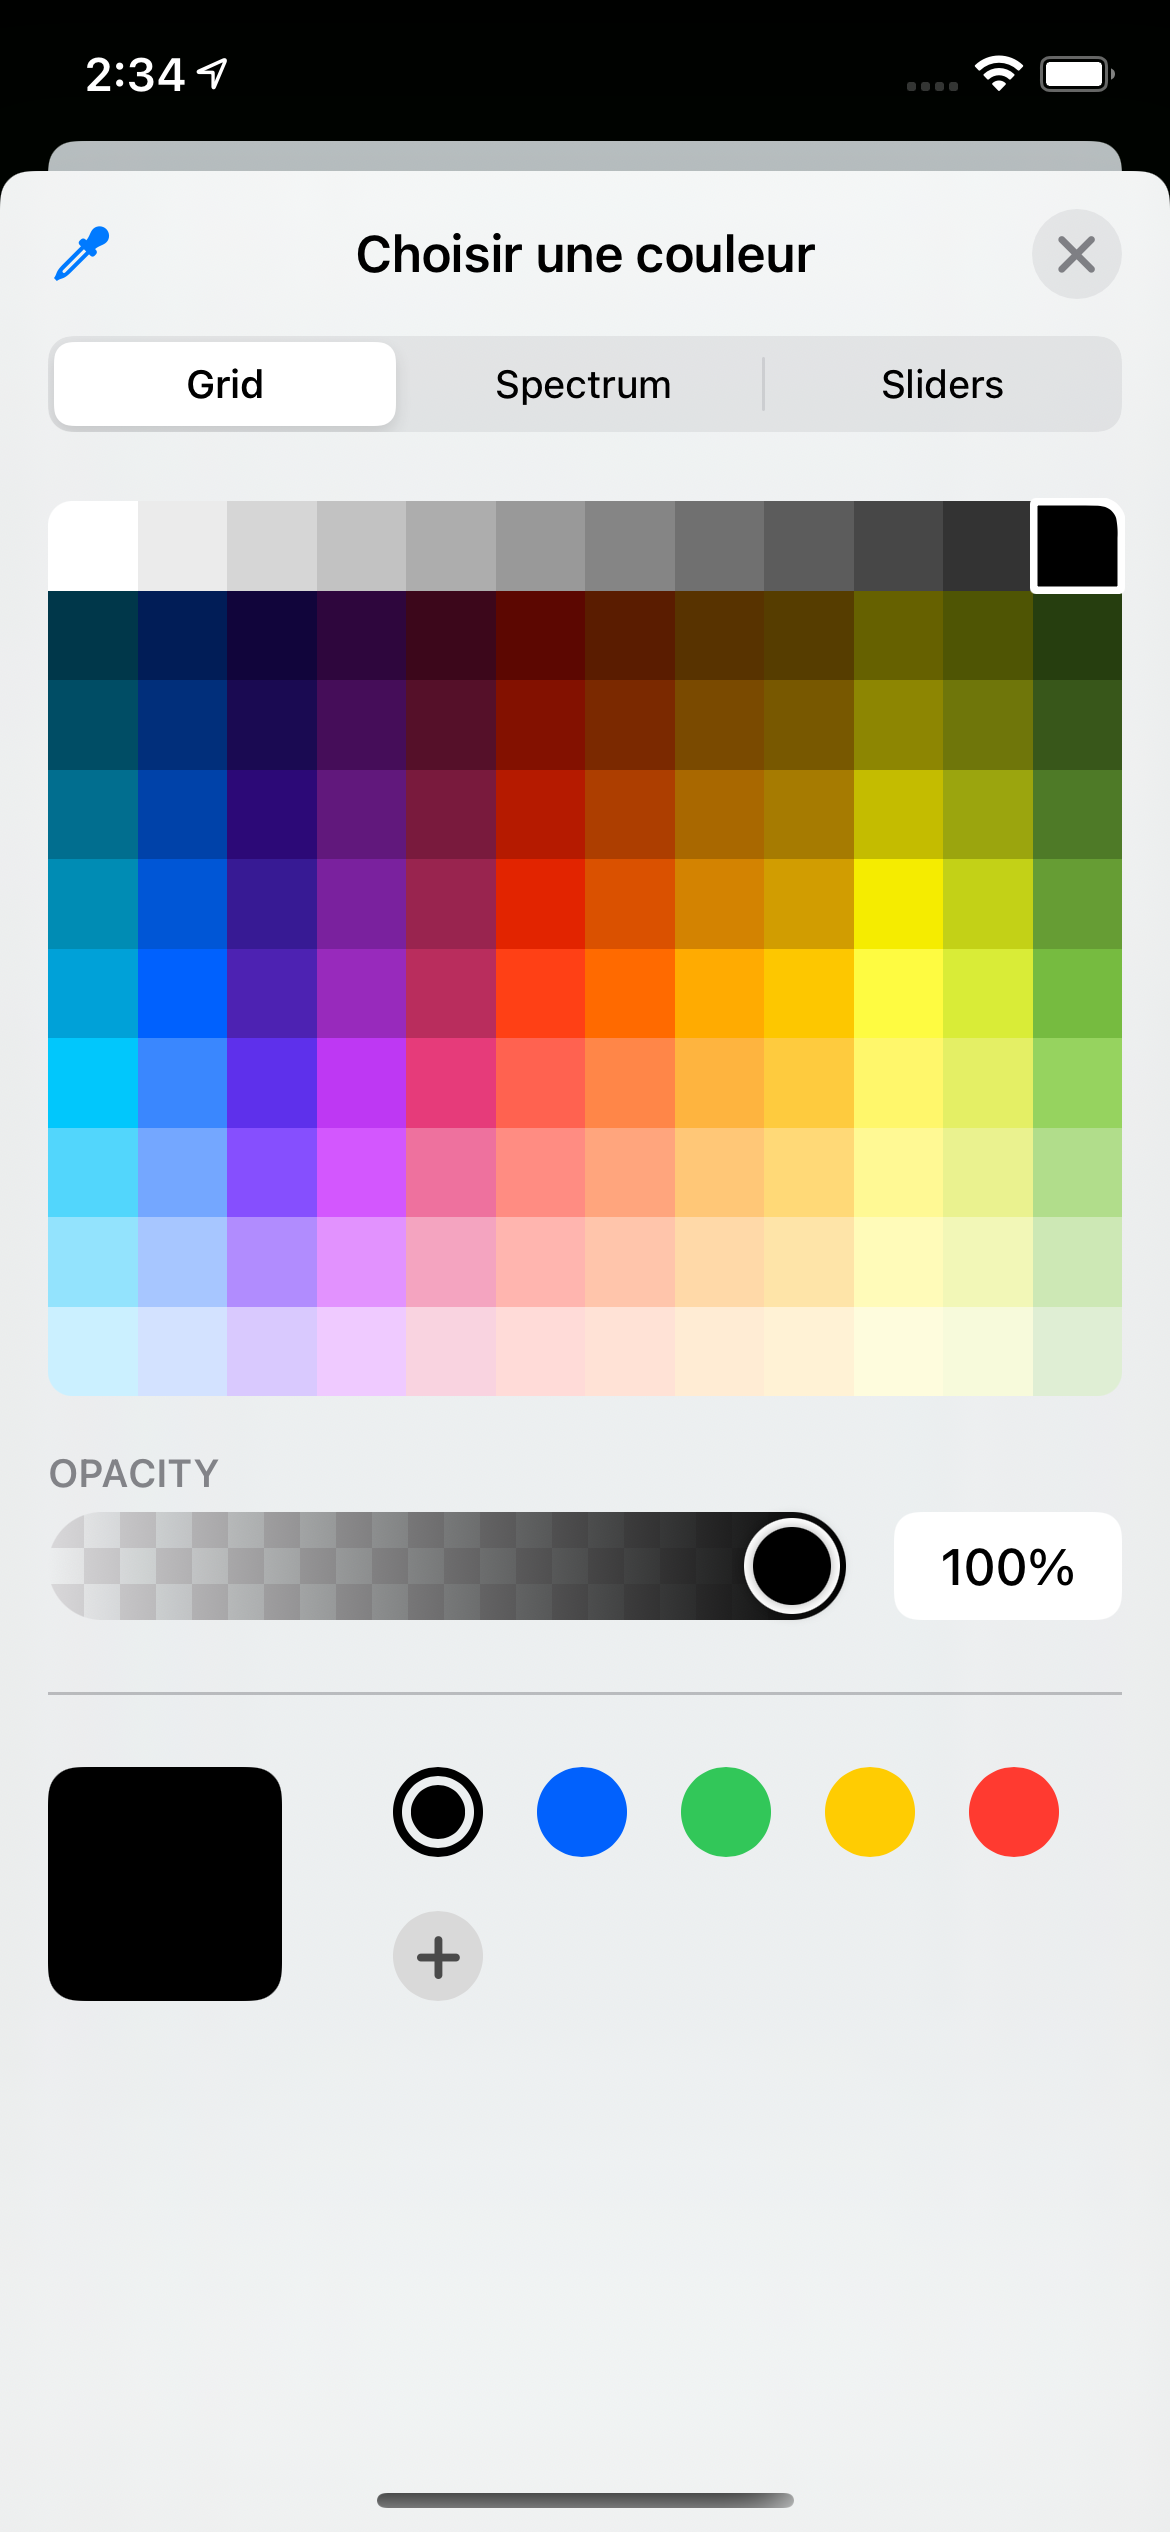
\includegraphics[height=7cm, width=3.5cm, scale=0.5]{setting_appearance.png}
      \end{tabular} \\
    \end{tabular}
  \end{frame}

  \begin{frame}
    \frametitle{Architecture du code : apparence}

    \begin{center}
      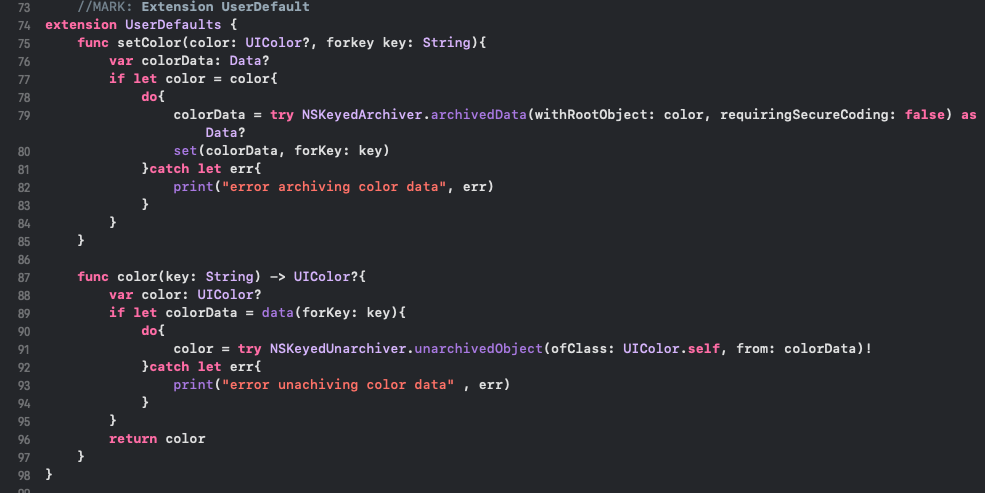
\includegraphics[height=70mm, width=120mm, scale=0.5]{colorPicker(iOS).png}
    \end{center}

  \end{frame}
  



\subsection{Paramètres : langues}
  \begin{frame}
    \frametitle{Architecture du code : langues}

    \begin{tabular}{cl}

      \begin{tabular}{c}
        \parbox{0.5\linewidth}{
          \begin{itemize}
            \item Utilisation du Bundle pour changer la langue
            \item Bundle : permet d'accéder à une ressource (fichier)
          \end{itemize}
        }
      \end{tabular} &
      
      \begin{tabular}{l}
        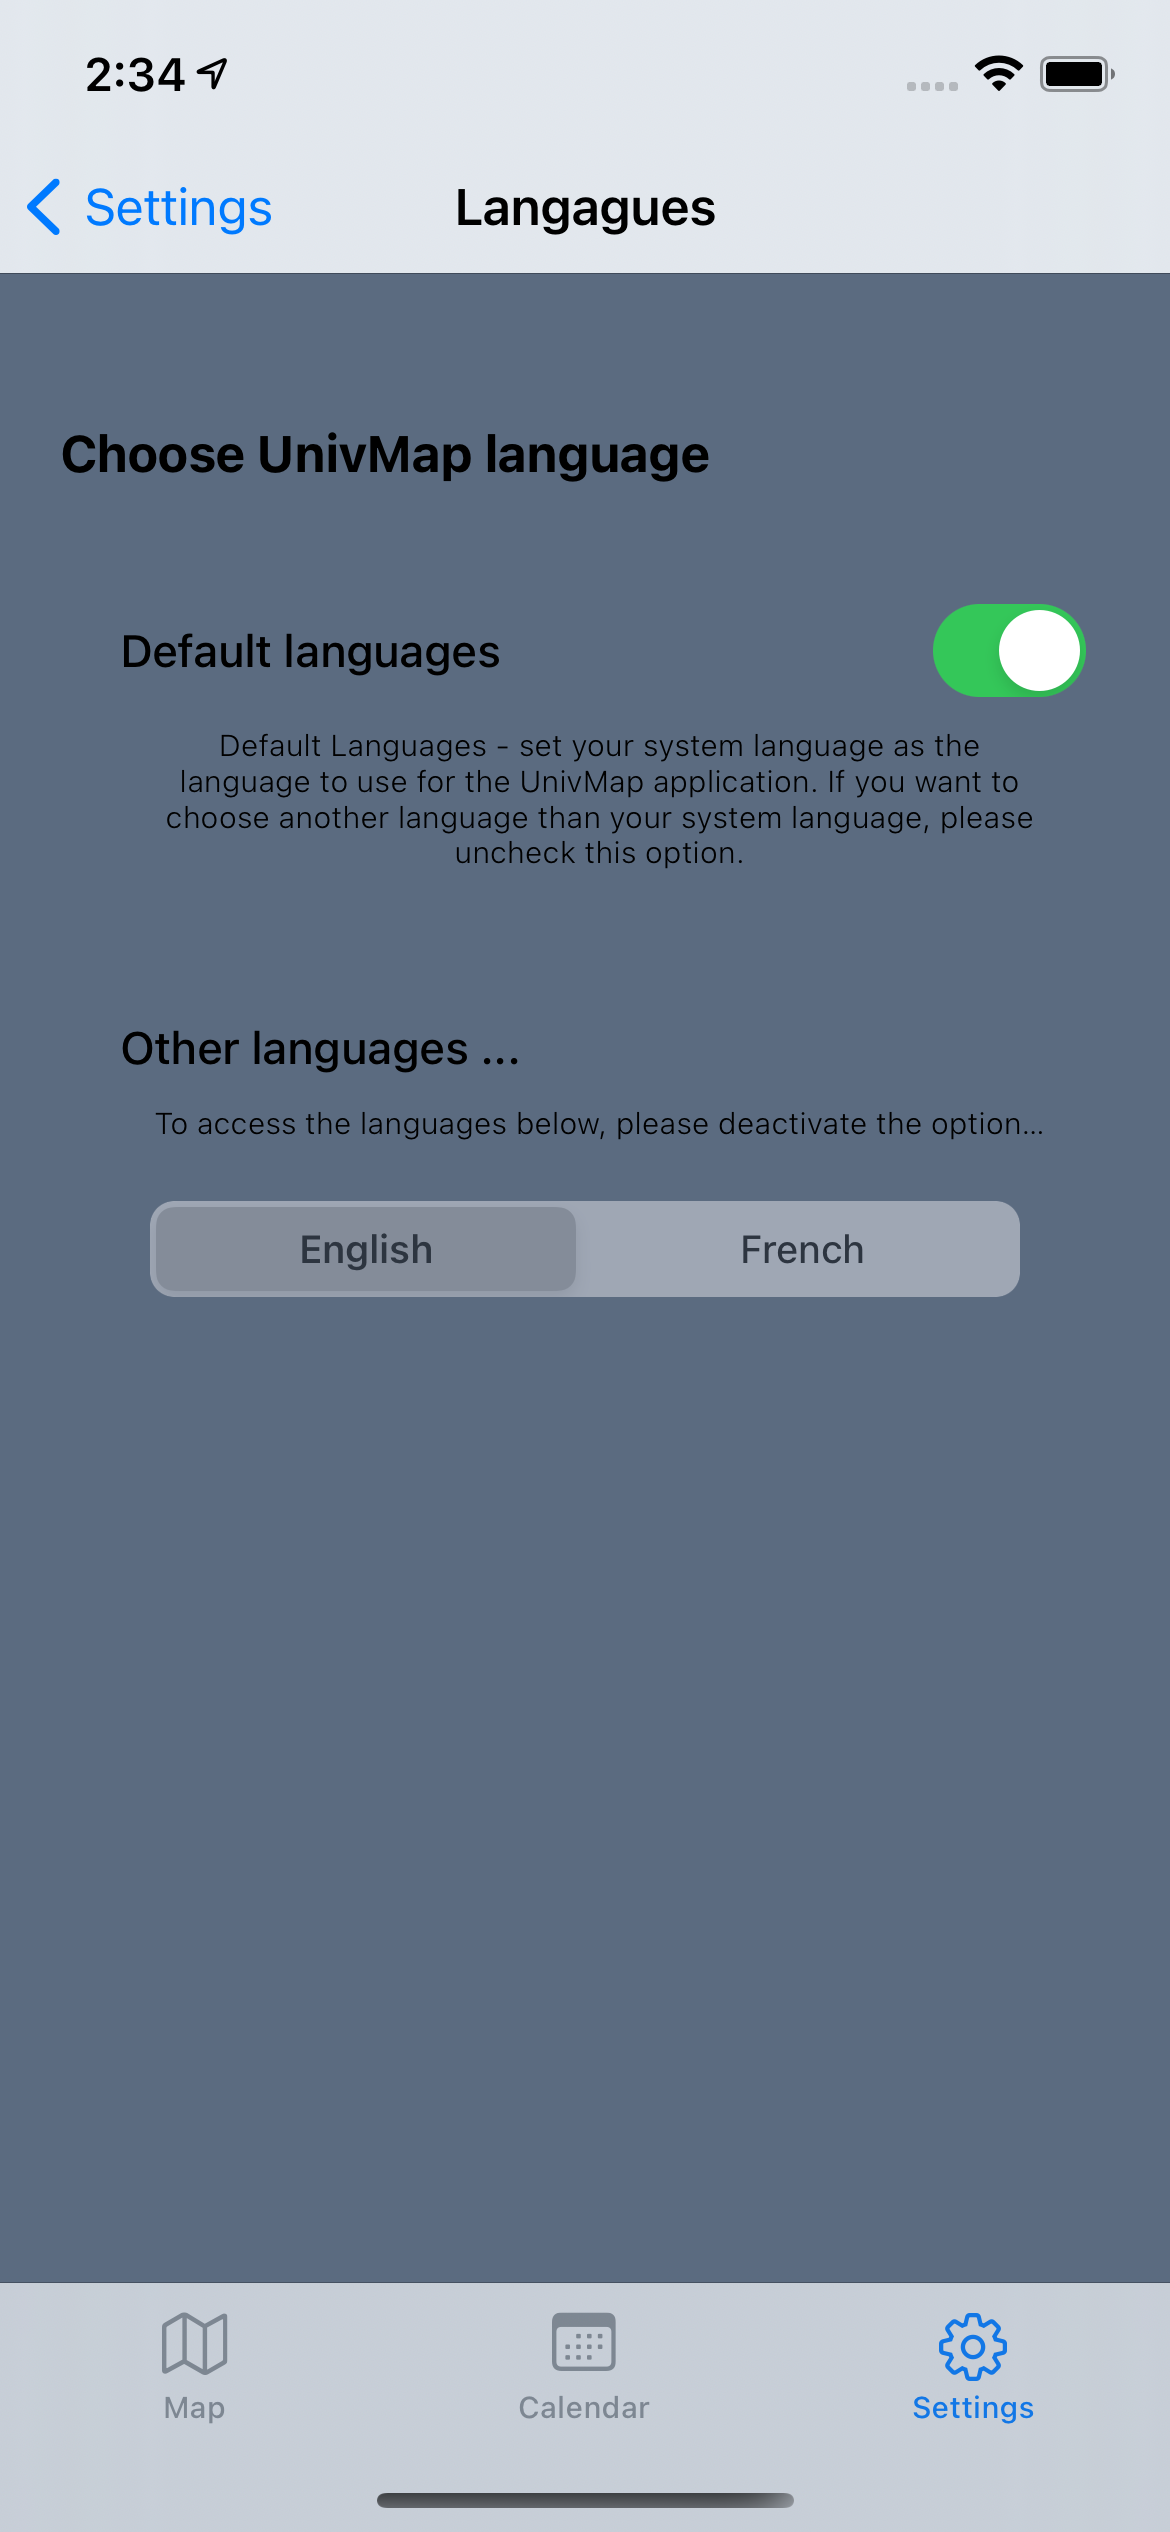
\includegraphics[height=7cm, width=3.5cm, scale=0.5]{setting_languageOn.png}
      \end{tabular} \\
    \end{tabular}
  \end{frame}

  \begin{frame}
    \frametitle{Architecture du code : langues}

    \begin{center}
      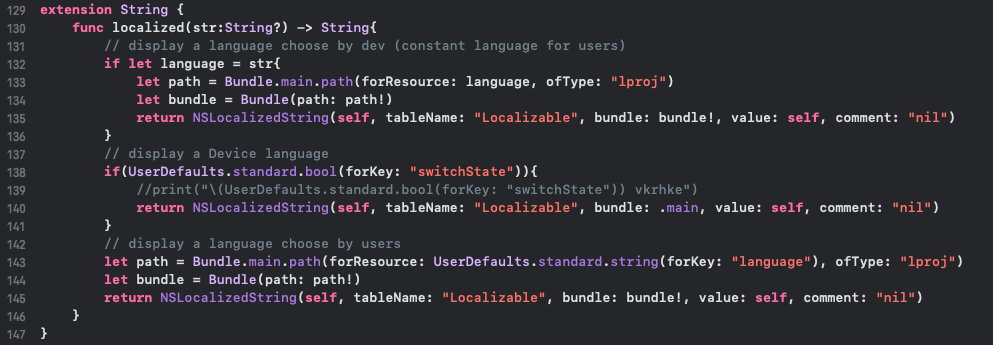
\includegraphics[height=55mm, width=120mm, scale=0.5]{language(iOS).png}
    \end{center}

  \end{frame}


% ****************************************************************************************************************************************
% *************************************                      Quelques difficultés                      ***********************************
% ****************************************************************************************************************************************
%
%
%%%%%%%%%%%%%%%%%%%%%%%%%%%%%%%%%%%%%%%%%%%%%%%%%%%%%%%%%%%%%%%%%%%%%%%%%%%%%
\section{Quelques difficultés}
%%%%%%%%%%%%%%%%%%%%%%%%%%%%%%%%%%%%%%%%%%%%%%%%%%%%%%%%%%%%%%%%%%%%%%%%%%%%%
%
%
\begin{frame}
  \frametitle{Quelques difficultés}
  \begin{itemize}
    \item Apprendre l'utilisation des API
    \item Comprendre les documentations
    \item Prise en main de Git
    \item Implémentation de Firebase sur iOS
    \item Changement de langues sur iOS
    \item Android : utilisation de fragment pour la navigation (crash de l'application)
  \end{itemize}
\end{frame}




% ****************************************************************************************************************************************
% *************************************                      UnivMap 2.0 : À Suivre                    ***********************************
% ****************************************************************************************************************************************
%
%
%%%%%%%%%%%%%%%%%%%%%%%%%%%%%%%%%%%%%%%%%%%%%%%%%%%%%%%%%%%%%%%%%%%%%%%%%%%%%
\section{UnivMap 2.0 : À Suivre}
%%%%%%%%%%%%%%%%%%%%%%%%%%%%%%%%%%%%%%%%%%%%%%%%%%%%%%%%%%%%%%%%%%%%%%%%%%%%%
%
%
\begin{frame}
  \frametitle{UnivMap 2.0 : À Suivre}

  \begin{itemize}
    \item Choix du planning selon une filière
    \item Notification lorsque l'emploi du temps est modifié
    \item Un onglet accueil afin d'être redirigé vers d'autres plateformes de l'Université
    \item Ajout de filtre pour la carte pour n'afficher que le contenu voulu
    \item Un système permettant de rechercher des salles
  \end{itemize}


\end{frame}



% ****************************************************************************************************************************************
% *************************************                           Conclusion                           ***********************************
% ****************************************************************************************************************************************
%
%
%%%%%%%%%%%%%%%%%%%%%%%%%%%%%%%%%%%%%%%%%%%%%%%%%%%%%%%%%%%%%%%%%%%%%%%%%%%%%
\section{Conclusion}
%%%%%%%%%%%%%%%%%%%%%%%%%%%%%%%%%%%%%%%%%%%%%%%%%%%%%%%%%%%%%%%%%%%%%%%%%%%%%
%
%
\begin{frame}
  \frametitle{Conclusion}

  \begin{center}
    
\includegraphics[width=35mm, scale=0.5]{UnivMap-logo500x500.png}
  \end{center}

  \begin{itemize}
    \item Appréhension sur l'idée de l'application
    \item Travail de groupe : communication, entraide étaient très important
    \item L'ambition et la persévérance d'atteindre cette objectif
  \end{itemize}
\end{frame}
%
%
\end{document}
